\documentclass[aps,prd,10pt,twocolumn,superscriptaddress,nofootinbib,floatfix,longbibliography,showpacs,showkeys]{revtex4-2}

\usepackage[T1]{fontenc}
\usepackage[utf8]{inputenc}
\usepackage{amsmath,amssymb,amsfonts,mathtools}
\usepackage{amsthm}
\usepackage{enumitem}
\usepackage{graphicx}
\usepackage{orcidlink}
\usepackage{xurl}
\hypersetup{colorlinks=true,linkcolor=blue!60!black,citecolor=blue!60!black,urlcolor=blue!60!black}

\theoremstyle{plain}
\newtheorem{theorem}{Theorem}
\newtheorem{proposition}{Proposition}
\newtheorem{lemma}{Lemma}
\newtheorem{corollary}{Corollary}
\theoremstyle{definition}
\newtheorem{definition}{Definition}
\newtheorem{hypothesis}{Hypothesis}
\theoremstyle{remark}
\newtheorem{remark}{Remark}

\newcommand{\bC}{\mathbb{C}}
\newcommand{\bR}{\mathbb{R}}
\newcommand{\bZ}{\mathbb{Z}}
\newcommand{\bE}{\mathbb{E}}
\newcommand{\cA}{\mathcal{A}}
\newcommand{\cB}{\mathcal{B}}
\newcommand{\cL}{\mathcal{L}}
\newcommand{\cN}{\mathcal{N}}
\newcommand{\Res}{\operatorname{Res}}
\newcommand{\rk}{\operatorname{rank}}
\newcommand{\im}{\operatorname{im}}
\newcommand{\erf}{\operatorname{erf}}
\newcommand{\erfc}{\operatorname{erfc}}
\newcommand{\Pt}{P^{(2)}}
\newcommand{\Ps}{P^{(0)}}
\newcommand{\dd}{\mathrm{d}}

%% The Zenodo record for the code archive.  Until the archive is deposited,
%% leave \zenodofalse: the Data Availability section then cites the code as
%% supplied with the article and makes no claim about a repository.  Once the
%% identifier is minted, set \zenodotrue and put it in \zenododoi.
\newif\ifzenodo
\zenodofalse
\newcommand{\zenododoi}{10.5281/zenodo.0000000}

\hbadness=5000
\emergencystretch=1.2em

\begin{document}

\title{Brane cluster gases and ghost-free form factors for quantum gravity}

\author{Deep Bhattacharjee\,\orcidlink{0000-0003-0466-750X}}
\email[Corresponding author: ]{itsdeep@live.com}
\affiliation{Formerly, Electro-Gravitational Space Propulsion Laboratory (EGSPL), Bhubaneswar, Odisha 751030, India}

\author{Priyabrata Mandal\,\orcidlink{0000-0001-6472-6239}}
\email{priyabrata@manit.ac.in}
\affiliation{Department of Mathematics, Bioinformatics and Computer Applications, Maulana Azad National Institute of Technology Bhopal, Bhopal 462003, India}

\author{Ushashi Bhattacharya\,\orcidlink{0009-0002-2254-3914}}
\email{rai.bhattacharya.in@gmail.com}
\affiliation{Formerly, National Taiwan University, Taipei 106319, Taiwan}

\date{\today}

\begin{abstract}
A graviton crossing a network of branes meets them one after another, and transmission amplitudes for successive traversals compose by multiplication, with corrections of second order in the single-brane reflectivity. A finite arrangement of $N$ branes therefore dresses the graviton kinetic operator by a polynomial form factor carrying one linear factor per brane. Every zero of that polynomial is a pole of the spin-two propagator, and we prove that the residues at the massive poles sum to $-1$, so they cannot all belong to healthy states; for real masses they alternate in sign beginning with a negative one. Replacing the arrangement by a Poisson gas replaces the product by its expectation, which is the probability generating functional of the process and hence the exponential of an entire function. An exponential has no zeros, so the averaged propagator retains one pole, at $p^2=0$, with residue $+1$. We keep this annealed statement separate from the quenched propagator of a frozen realization, which keeps its poles. For form factors of polynomial growth the superficial degree of divergence of a connected graph is $(2+2n)+(D-2-2n)L$, a function of the loop order alone, negative for every $L\ge2$ once $n\ge D$. For the Gaussian form factor the Euclidean propagator is an incomplete gamma function, finite at the origin; the Newtonian potential is $-(Gm/r)\erf(Mr/2)$; the linearized field satisfies $2|\Phi|<1$ at all radii precisely when $m<\sqrt{\pi}/(2GM)$; and the graviton is massless and luminal at every wavenumber. The same form factor raises the lower limit of every Schwinger parameter to $1/M^{2}$, which removes the ultraviolet region at every loop order when the vertices are polynomially bounded. Statements about ghosts refer throughout to the pole content of the tree-level propagator, not to unitarity of the interacting theory.
\end{abstract}

\keywords{nonlocal gravity; brane intersections; Poisson processes}
\makeatletter\def\@pacs@name{2020 MSC: }\makeatother
\pacs{Primary 83C45; Secondary 81T15, 60G55, 30D15}

\maketitle

\section{Introduction}
\label{sec:intro}

Perturbative quantum general relativity breaks down in a way that is visible from the power counting alone. The graviton propagator falls as $p^{-2}$, the vertices grow as $p^{2}$, and an $L$-loop graph in four dimensions has superficial degree of divergence $2+2L$, which increases without bound. Pure gravity is finite on shell at one loop but not once matter is added \cite{tHooftVeltman1974}, and at two loops the counterterm is nonzero \cite{GoroffSagnotti1986}. Of the two standard remedies, one adds curvature-squared terms, which flatten the propagator to $p^{-4}$ and render the theory renormalizable at the cost of a massive spin-two excitation of negative residue \cite{Stelle1977}; the other looks for a non-perturbative fixed point of the two-derivative action \cite{Weinberg1979,Reuter1998}. A third possibility, whose mathematical core is older than either, replaces the kinetic operator by an entire function of the d'Alembertian, $p^2\mapsto p^2e^{H(p^2)}$ \cite{Efimov1967,Krasnikov1987,Kuzmin1989,Tomboulis1997,BiswasMazumdarSiegel2006,BGKM2012,Modesto2012}. The propagator then has no pole except the massless one, and for suitable $H$ the loop integrands are damped.

In that third line of work the exponential is where the construction starts: a function $e^{H}$ is written down, its zero-free character is noted, and its consequences are developed. We address the step before that one. An exponential form factor is a strong assumption, and nothing in the usual presentation says why the ultraviolet completion should supply an exponential when any finite number of higher-derivative corrections produces a polynomial. The answer we give is statistical. Multiplicative contributions from independently placed scatterers exponentiate, because the expectation of a product over a Poisson process is the exponential of an integral, and that integral is the probability generating functional itself, not an approximation to it. On this reading the exponential is what a random medium generically produces, and the polynomial case is recovered exactly when the medium is frozen or finite.

Our question is where such a form factor might come from, and what can be established once it is there. The mechanism we examine is a network of branes. Hypersurfaces in general position generate strata, the intersections of one, two, three or more of them, indexed by the subsets of the collection. If the coupling of the metric to the branes is multiplicative over these strata, the graviton kinetic operator acquires a sum over subsets, and such a sum factorizes into binomials. A deterministic arrangement of $N$ branes therefore gives
\begin{equation}
\label{eq:poly-intro}
a(z)=\prod_{i=1}^{N}\Bigl(1+\frac{w_i\,z}{M^2}\Bigr),\qquad z=-\Box,
\end{equation}
a polynomial of degree $N$ whose zeros are poles of the propagator. We show below that the residues at those poles are constrained to sum to $-1$, so at least one of them is unhealthy. If instead the branes form a gas, by which we mean a Poisson point process on the space of branes with intensity measure $\Lambda$, the expectation of the same product is
\begin{equation}
\label{eq:exp-intro}
\bE\prod_{i}\Bigl(1+\frac{w_i z}{M^2}\Bigr)=\exp\Bigl(\frac{z}{M^2}\int w\,\dd\Lambda\Bigr),
\end{equation}
the probability generating functional of the process. This is an exponential of a linear function, and it vanishes nowhere.

Equation \eqref{eq:exp-intro} averages the kinetic operator and not the propagator, and the two are not interchangeable. A gas whose fluctuations are fast compared with the graviton can be integrated out into an effective quadratic action carrying the averaged operator, which has no zeros; a gas frozen into one realization leaves the polynomial \eqref{eq:poly-intro} in place together with its poles. Remark~\ref{rem:annealed} makes the separation precise, and Theorem~\ref{thm:sumrule} quantifies what the frozen case costs. Couplings more general than the linear one give $\exp\int w(x,z)\,\dd\Lambda(x)$, an exponential of an entire function of $z$, and this is the class of form factors whose propagator carries a single pole.

Before summarizing what follows we fix a term. A form factor is called ghost free here when the spin-two propagator it produces has one pole, at $p^2=0$, with positive residue. The phrase refers to the pole content of the tree-level propagator and carries no claim about unitarity of the interacting theory. That limitation is taken up again in Sec.~\ref{sec:discussion}.

Three results are established. The first concerns the pole content, which turns out to be a dichotomy with a sum rule attached. If the form factor $a$ is entire with $a(0)=1$ and has a zero, the propagator has a pole there. If $a$ is a polynomial of degree $N$ there are $N$ such poles counted with multiplicity, and their residues add to $-1$ (Theorem~\ref{thm:sumrule}). They cannot then all be healthy: for real positive masses they alternate in sign beginning with a negative one, and in general at least one has negative real part. If $a$ has no zero, then $a=e^{H}$ with $H$ entire, the propagator retains a single pole at $p^2=0$ with residue $+1$, and the graviton is massless and luminal at every wavenumber (Theorem~\ref{thm:dichotomy}). The second result is that a Poisson process of branes with multiplicative couplings has an expected form factor equal to the exponential of an entire function (Theorem~\ref{thm:poisson}); nothing is truncated in the sum over strata, and the $1/K!$ responsible for the exponential is the $1/K!$ of the factorial moment measures of the process. The third is the power counting, which closes under a growth condition. If $a(p^2)\sim p^{2n}$ and the vertex form factors grow with it as diffeomorphism invariance requires, the superficial degree of divergence of a connected graph in $D$ dimensions is $(2+2n)+(D-2-2n)L$, a function of the loop order alone. In four dimensions it is negative for $L>(n+1)/(n-1)$, so the divergent loop orders are $\{1,2,3\}$ at $n=2$, $\{1,2\}$ at $n=3$ and $\{1\}$ for every $n\ge4$; in $D$ dimensions only one-loop graphs diverge once $n\ge D$ (Theorem~\ref{thm:power}). The growth condition is a real restriction and we carry it explicitly as Hypothesis~\ref{hyp:growth}. The Gaussian form factor violates it, and for that case the counting is silent.

The Gaussian form factor $a=e^{-\Box/M^2}$ is the case Theorem~\ref{thm:power} excludes, and we treat it separately. In the parametric representation its effect is to raise the lower limit of every Schwinger parameter from zero to $1/M^2$, which deletes the corner of parameter space that carries the ultraviolet divergences and leaves the first Symanzik polynomial bounded below by $t(G)M^{-2L}$, with $t(G)$ the number of spanning trees of the graph (Theorem~\ref{thm:noUV}). With vertices polynomial in the momenta this removes the ultraviolet divergence of every graph at every loop order, and the one-loop bubble is finite with the closed form \eqref{eq:bubble0} at zero external momentum. The vertices of a gravitational theory are not polynomially bounded, which is where the analysis of Talaganis, Biswas and Mazumdar \cite{Talaganis2015} takes over, and Remark~\ref{rem:vertices} says exactly how much of the problem the propagators settle on their own.

Alongside these we work out what the same form factor implies classically. Its Euclidean propagator can be written in every dimension as an incomplete gamma function, and that function is bounded at the origin by $M^{D-2}/(2^{D-1}\pi^{D/2}(D-2))$. The Newtonian potential becomes $-(Gm/r)\erf(Mr/2)$, which stays finite at $r=0$ where the Newtonian potential diverges. The linearized field satisfies $2|\Phi|<1$ at all radii precisely when $m<\sqrt\pi/(2GM)$. This last condition is the linearized form of the horizon-formation threshold Frolov \cite{Frolov2015} obtained in the same approximation, and on its own it says nothing about the nonlinear solution. Finally, a laboratory test of the inverse-square law at separation $r$ and precision $\epsilon$ bounds $M>(2/r)\erfc^{-1}(\epsilon)$.

The brane picture enters through one physical input, and it should be stated precisely. Multiplicativity is not among the assumptions. Amplitudes for successive traversals of a stack compose by multiplication, which is Lemma~\ref{lem:compose}, and the corrections to the product are second order in the single-brane reflection amplitudes. What is assumed is that those reflections are small and that the single-brane forward amplitude may be truncated after its first derivative correction, which is Hypothesis~\ref{hyp:mult}, and this is the same dilute regime that makes a Poisson description of the positions appropriate. Everything downstream is a theorem about entire functions, about graphs, or about the Poisson process, so a reader who does not accept the brane interpretation still keeps those theorems. We make no claim that a brane gas is the only route to a nonlocal form factor, and we prove nothing about unitarity beyond the residue statement at tree level. An earlier preprint by one of us with other collaborators \cite{Bhattacharjee2025brane} proposed brane clustering as an ultraviolet completion, with several of its structures asserted rather than derived; the present paper replaces that proposal with the Poisson mechanism and with proofs, and adds the sum rule, the closed-form propagator and the mass threshold.

The paper is arranged as follows. Section~\ref{sec:arrangements} sets up brane arrangements, their nerve complex and their integral charges. Section~\ref{sec:gas} derives the polynomial and the exponential form factors. Section~\ref{sec:propagator} writes down the dressed propagator and its Ward identity, Sec.~\ref{sec:poles} proves the dichotomy and the sum rule, Sec.~\ref{sec:power} the power counting, and Sec.~\ref{sec:gaussian} the classical consequences of the Gaussian form factor. Section~\ref{sec:compare} places the standard frameworks on a single axis, Sec.~\ref{sec:verification} describes the code that recomputes every number, and Sec.~\ref{sec:discussion} states what remains open. Appendix~\ref{app:conventions} fixes the conventions, Appendix~\ref{app:stress} carries out the variation of the form-factor term, and Appendix~\ref{app:poisson} collects the two Poisson identities used in Sec.~\ref{sec:gas}.

\begin{figure*}[t]
\centering
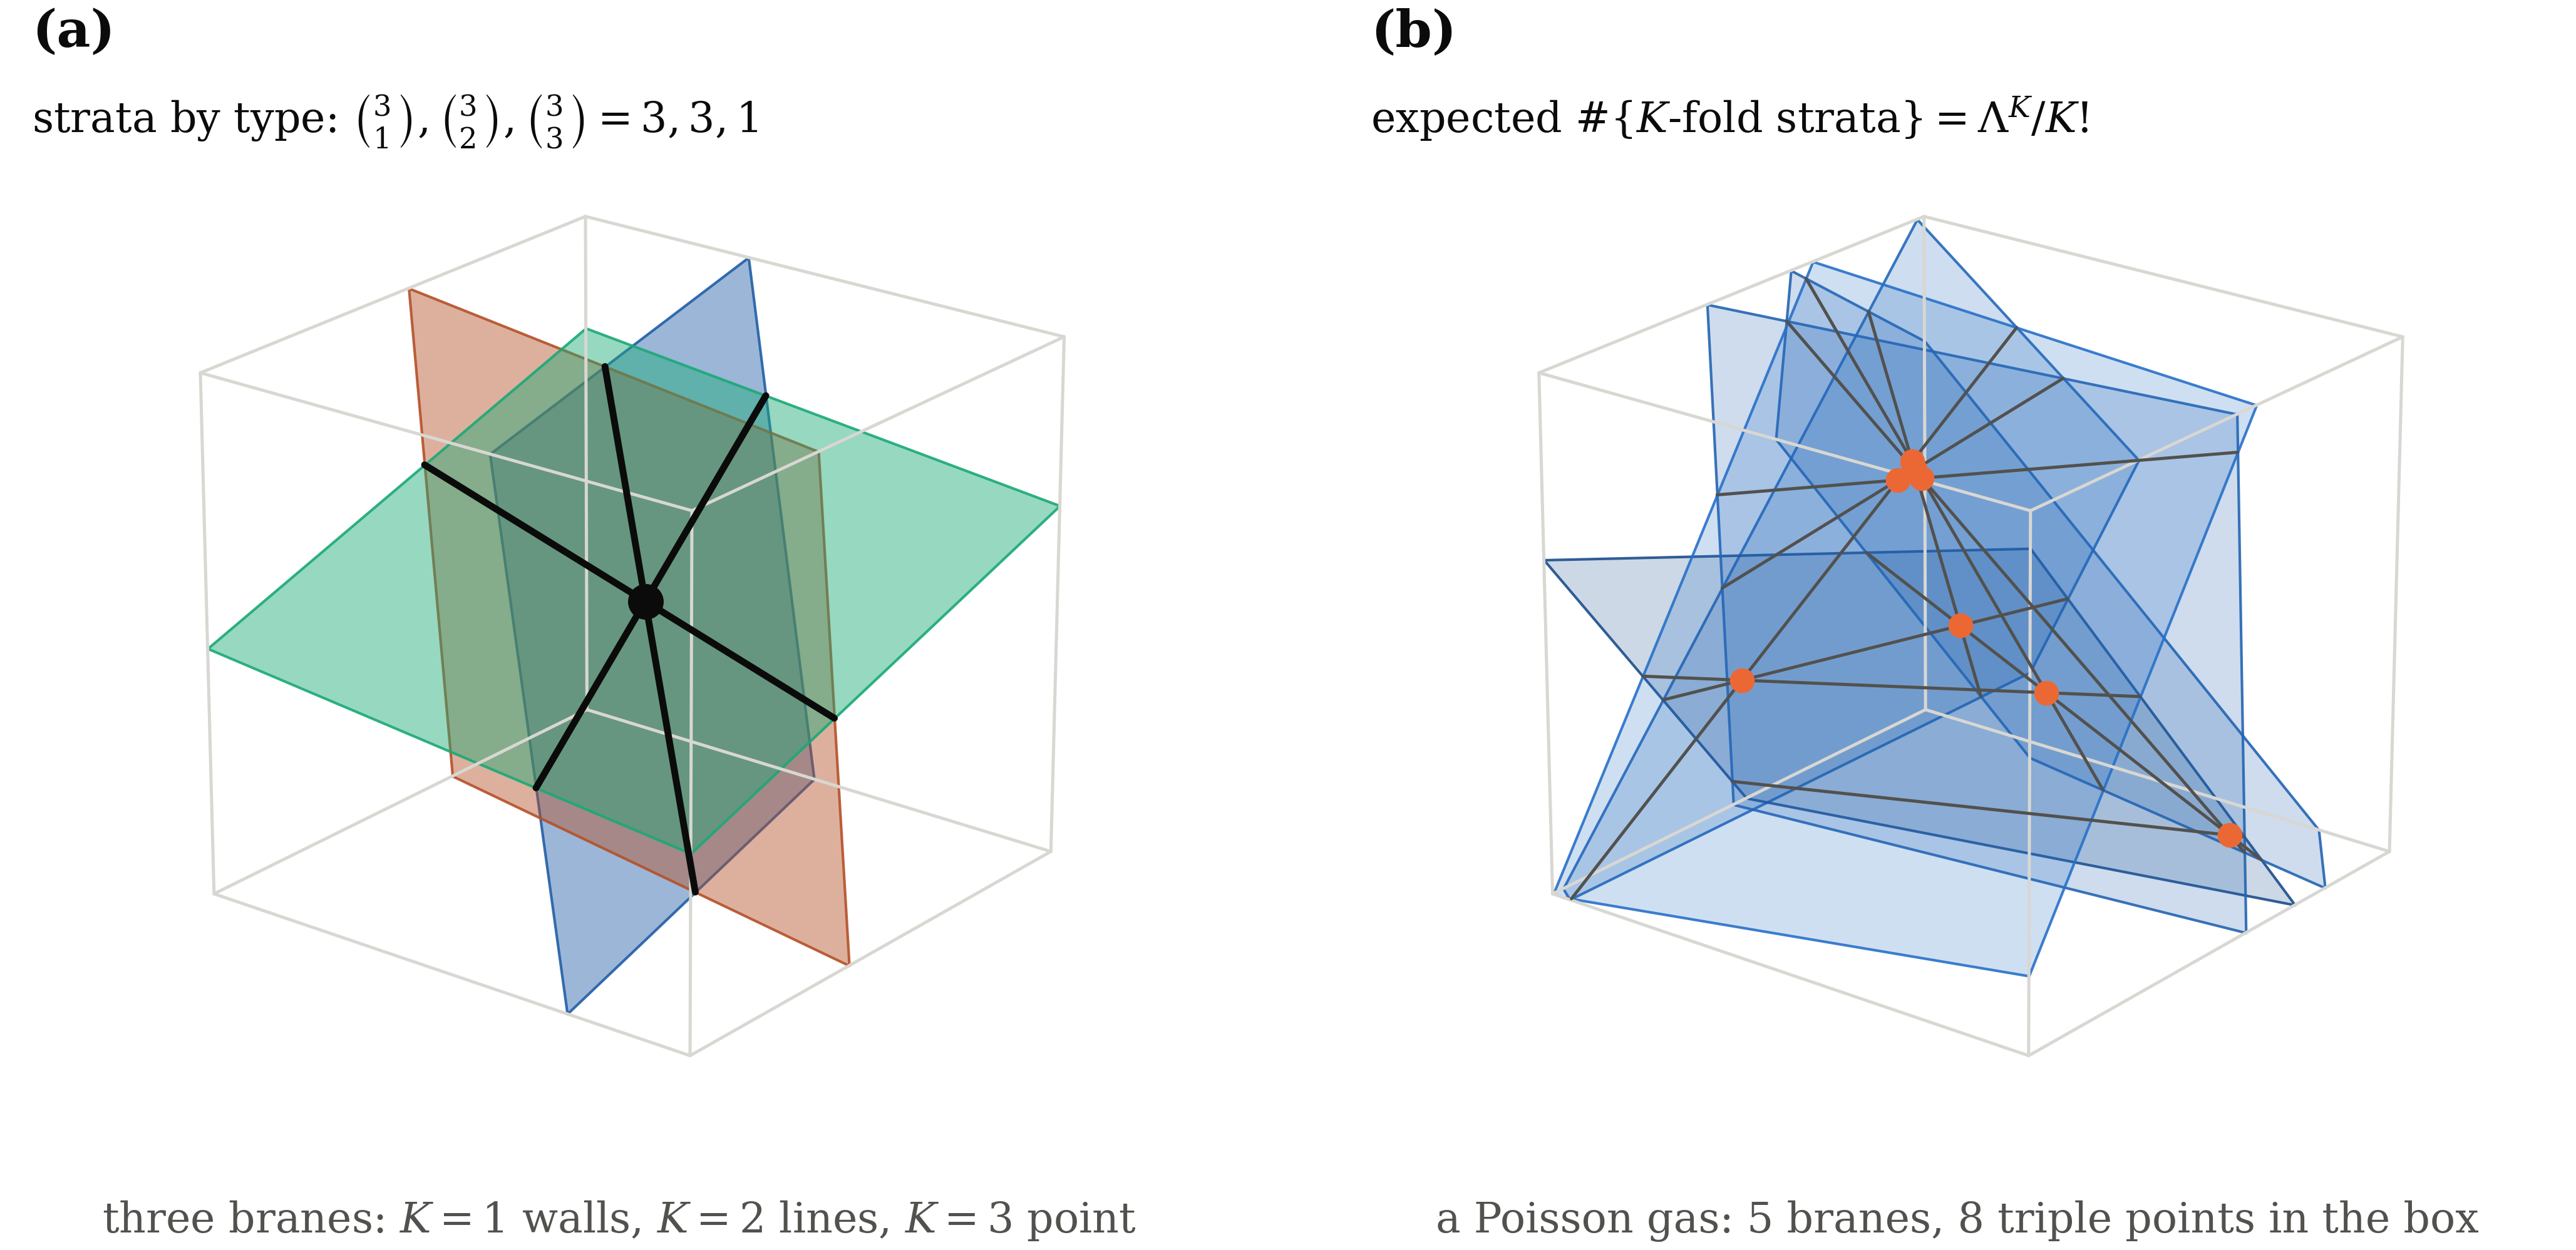
\includegraphics[width=\textwidth]{figs/fig01_arrangement.png}
\caption{(a) Three transverse branes in a cube of three-space: the strata are the three walls, the three lines, and one point, indexed by the nonempty subsets of the arrangement. (b) A Poisson gas of branes in the same box, with its pairwise intersection lines and its triple points; the expected number of $K$-fold strata is $\Lambda^K/K!$ for a gas of intensity $\Lambda$, which is the source of the exponential in Theorem~\ref{thm:poisson}.}
\label{fig:arrangement}
\end{figure*}

\section{Brane arrangements}
\label{sec:arrangements}

\subsection{The nerve complex}

\begin{definition}
\label{def:arrangement}
A \emph{brane arrangement} in a smooth oriented $D$-manifold $X$ is a finite collection $\cB=\{B_1,\dots,B_N\}$ of closed oriented submanifolds in general position. Its \emph{strata} are the intersections $B_S=\bigcap_{i\in S}B_i$ over the subsets $S\subseteq\{1,\dots,N\}$ for which $B_S\neq\emptyset$; a stratum with $|S|=K$ is a \emph{$K$-cluster}. The \emph{nerve} of $\cB$ is the simplicial complex whose $k$-simplices are the sets $S$ with $|S|=k+1$ and $B_S\ne\emptyset$, and its chain complex $(C_\bullet,\partial)$ is the free abelian group on the strata with
\begin{equation}
\label{eq:boundary}
\partial[B_S]=\sum_{j=0}^{k}(-1)^{j}\,[B_{S\setminus\{s_j\}}],\qquad S=\{s_0<\cdots<s_k\}.
\end{equation}
\end{definition}

The smallest case with strata of every codimension is drawn in Fig.~\ref{fig:arrangement}(a): three transverse branes in a cube, whose seven nonempty strata are the three walls, the three lines and the point, indexed by the seven nonempty subsets. Panel (b) of the same figure replaces the three branes by a gas, which is the object of Sec.~\ref{sec:gas}.

\begin{proposition}
\label{prop:complex}
$\partial\circ\partial=0$, so the homology $H_k(\cB)=\ker\partial_k/\im\partial_{k+1}$ is defined, and
\begin{equation}
\label{eq:euler}
\sum_{k}(-1)^k\rk C_k=\sum_k(-1)^k\rk H_k(\cB).
\end{equation}
If every nonempty stratum is contractible, $H_\bullet(\cB)$ is the homology of the union $\bigcup_iB_i$.
\end{proposition}

\begin{proof}
Applying \eqref{eq:boundary} twice, the term of $\partial\partial[B_S]$ in which the branes $s_j$ and $s_l$, $j<l$, have been removed appears twice: removing $s_j$ first contributes the sign $(-1)^j(-1)^{l-1}$, because after the removal of $s_j$ the brane $s_l$ sits in position $l-1$; removing $s_l$ first contributes $(-1)^l(-1)^j$. The two cancel. For \eqref{eq:euler} write $r_k=\rk\partial_k$; then $\rk H_k=\rk C_k-r_k-r_{k+1}$, and in the alternating sum each $r_k$ appears with the signs $(-1)^{k}$ and $(-1)^{k-1}$, so they cancel. The last statement is the nerve theorem \cite{Bauer2023}, applied to the cover of the union by the branes.
\end{proof}

The identity $\partial^2=0$ is a statement about orientations of subsets and holds for every arrangement in every dimension. The charges introduced next are integers for that reason and no other.

\subsection{Integral charges}

A $K$-cluster of an arrangement of hypersurfaces has codimension $K$, and the orientation bookkeeping of Proposition~\ref{prop:complex} makes its fundamental class $[B_S]\in H_{D-K}(X;\bZ)$ well defined; this class is its \emph{charge}; paired with a class in $H^{D-K}(X;\bZ)$ the charge is an integer, invariant under deformations of the branes through general position and independent of the metric, so it receives no perturbative correction.

\begin{proposition}
\label{prop:torus}
Let $X=T^D=\bR^D/\bZ^D$ and let $\Sigma_1=V_1/L_1$ and $\Sigma_2=V_2/L_2$ be subtori of complementary dimensions, $V_i\subset\bR^D$ the real span of a primitive sublattice $L_i\subset\bZ^D$, with $V_1\oplus V_2=\bR^D$. Assemble bases of $L_1$ and $L_2$ as the rows of a matrix $M\in\bZ^{D\times D}$, so that $\det M\ne0$. Then $\Sigma_1$ and $\Sigma_2$ meet transversally in exactly
\begin{equation}
\label{eq:detM}
\#(\Sigma_1\cap\Sigma_2)=|\det M|=[\bZ^D:L_1\oplus L_2]
\end{equation}
points, and this number is the evaluation of the cup product of their Poincar\'e duals on the fundamental class. For two closed curves on $T^2$ with primitive winding vectors $(p_1,q_1)$ and $(p_2,q_2)$ it is $|p_1q_2-p_2q_1|$.
\end{proposition}

\begin{proof}
A point of $\Sigma_1\cap\Sigma_2$ is a class $x+\bZ^D$ with $x\in V_1$ and $x\in V_2+\bZ^D$, that is $x=v_2+n$ with $v_2\in V_2$ and $n\in\bZ^D$. Since $V_1\oplus V_2=\bR^D$, every $n\in\bZ^D$ decomposes uniquely as $n=x-v_2$ with $x\in V_1$, $v_2\in V_2$, and two integer vectors $n,n'$ give the same point of $\Sigma_1\cap\Sigma_2$ exactly when $x-x'\in L_1$ and $v_2-v_2'\in L_2$, that is when $n-n'\in L_1\oplus L_2$. Hence $\Sigma_1\cap\Sigma_2$ is in bijection with $\bZ^D/(L_1\oplus L_2)$, a group of order $[\bZ^D:M^{\mathsf T}\bZ^D]$. By the Smith normal form $M=U\,\mathrm{diag}(d_1,\dots,d_D)\,V$ with $U,V$ unimodular \cite[Chapter~2]{Cohen1993}, the index is $\prod|d_i|=|\det M|$. Transversality is the condition $V_1\oplus V_2=\bR^D$. The identification with a cup product is Poincar\'e duality \cite[Chapter~I]{BottTu1982}. The two-torus law is the case $D=2$.
\end{proof}

\begin{proposition}[census]
\label{prop:census}
For the arrangement of the $D$ coordinate hypertori of $T^D$ the number of $K$-clusters is $\binom DK$ and the total number of strata is $2^D$, and
\begin{equation}
\label{eq:census}
\sum_{K=0}^{D}(-1)^K\binom DK=0=\chi(T^D).
\end{equation}
\end{proposition}

\begin{proof}
Any $K$ of the coordinate hypertori meet transversally in a single subtorus, so the $K$-clusters are the $K$-subsets. The binomial theorem at $x=1$ and $x=-1$ gives the two sums, and the second is the Euler characteristic of the product cell structure of $T^D$, whose $K$-cells are indexed by the same subsets.
\end{proof}

Figure~\ref{fig:torus} collects the two counts: the determinant law of Proposition~\ref{prop:torus} over every primitive pair of winding vectors with small entries, and the census of Proposition~\ref{prop:census} in a range of dimensions.

\begin{figure*}[t]
\centering
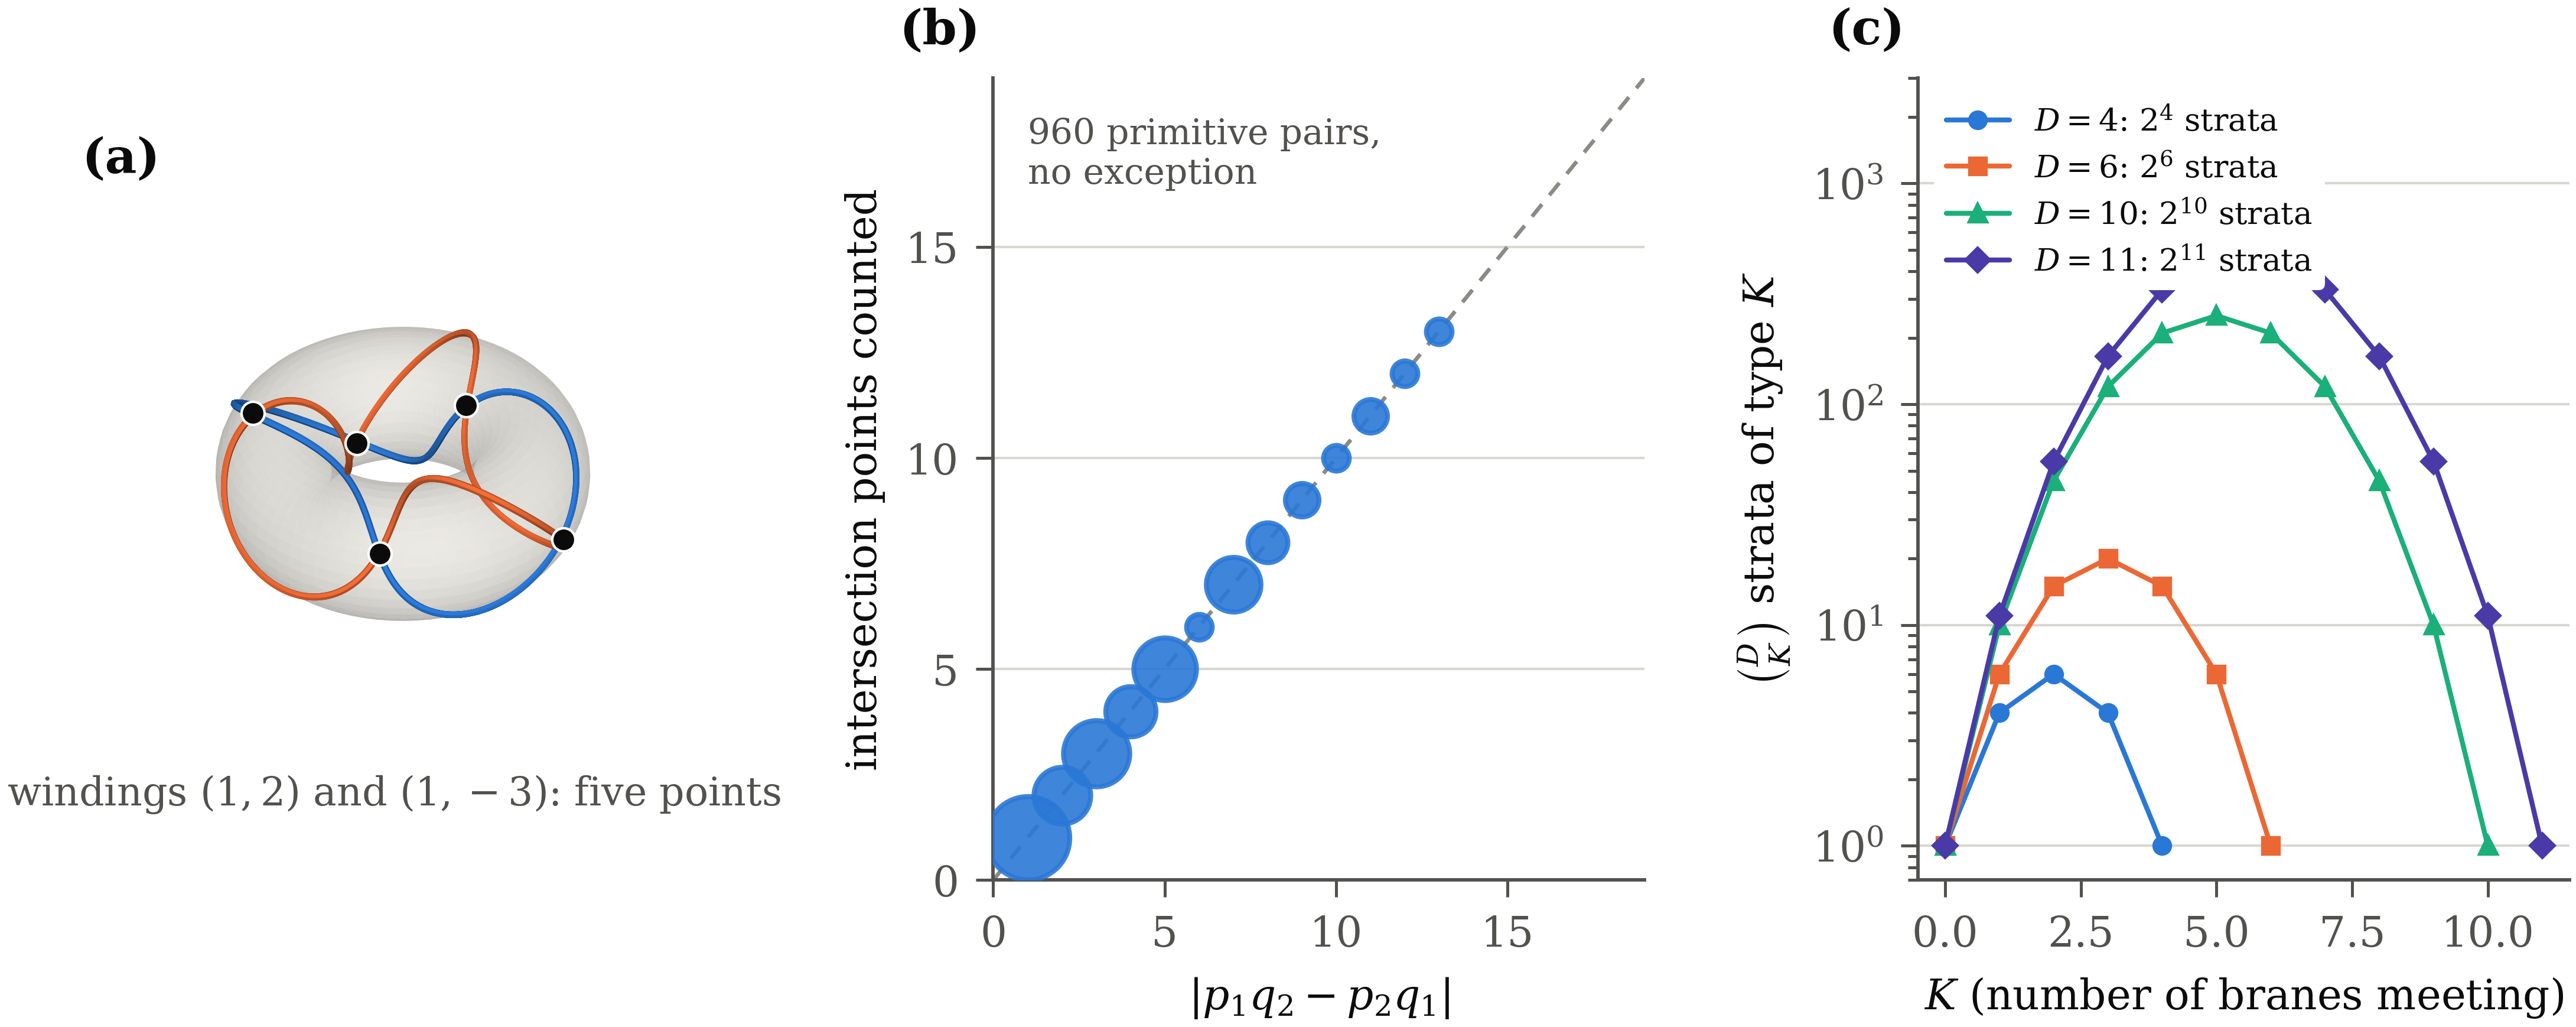
\includegraphics[width=\textwidth]{figs/fig02_torus.png}
\caption{(a) Two closed curves of winding numbers $(1,2)$ and $(1,-3)$ on a torus meet in exactly $|1\cdot(-3)-1\cdot2|=5$ points. (b) The determinant law of Proposition~\ref{prop:torus} on all $960$ pairs of primitive winding vectors with entries in $[-3,3]$; marker area grows with the number of pairs at each point. (c) The census of Proposition~\ref{prop:census} in several dimensions.}
\label{fig:torus}
\end{figure*}

\section{From arrangements to form factors}
\label{sec:gas}

\subsection{Multiplicativity as a composition law}
\label{sec:mult}

Let $h_{\mu\nu}$ be the graviton and let the quadratic part of its Euclidean action, before any coupling to branes, be $\tfrac12\int h\,K(p^2)\,h$ with $K(p^2)=p^2$ on the spin-two projector. The question is what the branes do to $K$, and a composition law settles it.

A graviton crossing the network meets the branes one after another, and amplitudes for successive traversals compose by multiplication, not by addition. This is the content of multiple scattering theory in the regime where the scatterers act independently \cite{Foldy1945,Lax1951}. We make that statement precise for a stack and then read off the form factor.

Write $t_i(p)$ and $r_i(p)$ for the forward transmission and reflection amplitudes of the single brane $B_i$, and let $\delta$ be the phase a mode of momentum $p$ accumulates between two consecutive branes.

\begin{lemma}[transmission amplitudes compose]
\label{lem:compose}
For two branes the transmission amplitude of the pair is
\begin{equation}
\label{eq:fabry}
t_{12}=\frac{t_1t_2}{1-r_1'r_2\,e^{2i\delta}},
\end{equation}
with $r_1'$ the reflection amplitude of the first brane seen from the right, which for a symmetric lossless brane is $-\overline{r_1}$. For $N$ branes,
\begin{equation}
\label{eq:product}
t_{1\cdots N}=\Bigl(\prod_{i=1}^{N}t_i\Bigr)\bigl(1+\mathcal E\bigr),
\qquad
|\mathcal E|\le C\!\!\sum_{i<j}|r_i||r_j|
\end{equation}
for a constant $C$ depending only on $N$ through the number of reflection paths, so the transmission factorizes whenever the reflection amplitudes are small.
\end{lemma}

\begin{proof}
A mode incident from the left is transmitted through the first brane, transmitted through the second, and in addition may be reflected any number of times between them. Summing the geometric series of round trips gives
\[
t_1t_2\sum_{n\ge0}\bigl(r_1'r_2e^{2i\delta}\bigr)^{n}=\frac{t_1t_2}{1-r_1'r_2e^{2i\delta}},
\]
which is \eqref{eq:fabry}; the series converges because $|r_1'r_2|<1$ for a lossless brane, where $|t_i|^2+|r_i|^2=1$. Iterating over the stack, every term of the expansion of $t_{1\cdots N}$ beyond $\prod_it_i$ contains at least one round trip, hence at least two reflection amplitudes, which gives the bound in \eqref{eq:product}.
\end{proof}

The two-point function of the graviton along the stack is the free one multiplied by $t_{1\cdots N}$, so the dressed kinetic operator is $p^2\prod_it_i^{-1}$. What remains is the single-brane factor. A brane is thin compared with the wavelengths of interest, so its forward amplitude admits a derivative expansion, and by parity in $p$ the expansion proceeds in powers of $p^2$:
\begin{equation}
\label{eq:derivexp}
t_i^{-1}(p)=1+\frac{w_ip^2}{M^2}+O\Bigl(\frac{p^4}{M^4}\Bigr),
\end{equation}
where $M$ is the scale set by the brane thickness and tension and $w_i\ge0$ is the dimensionless strength of brane $i$. The coefficient $w_i$ is a parameter of the model; the product structure in front of it is not. Figure~\ref{fig:transfer} shows where the product comes from and how accurate it is: panel (a) is the direct path together with the round trip that produces the leading correction, and panel (b) measures the error of \eqref{eq:product} against the transfer matrix of the stack, which composes every reflection exactly.

\begin{figure*}[t]
\centering
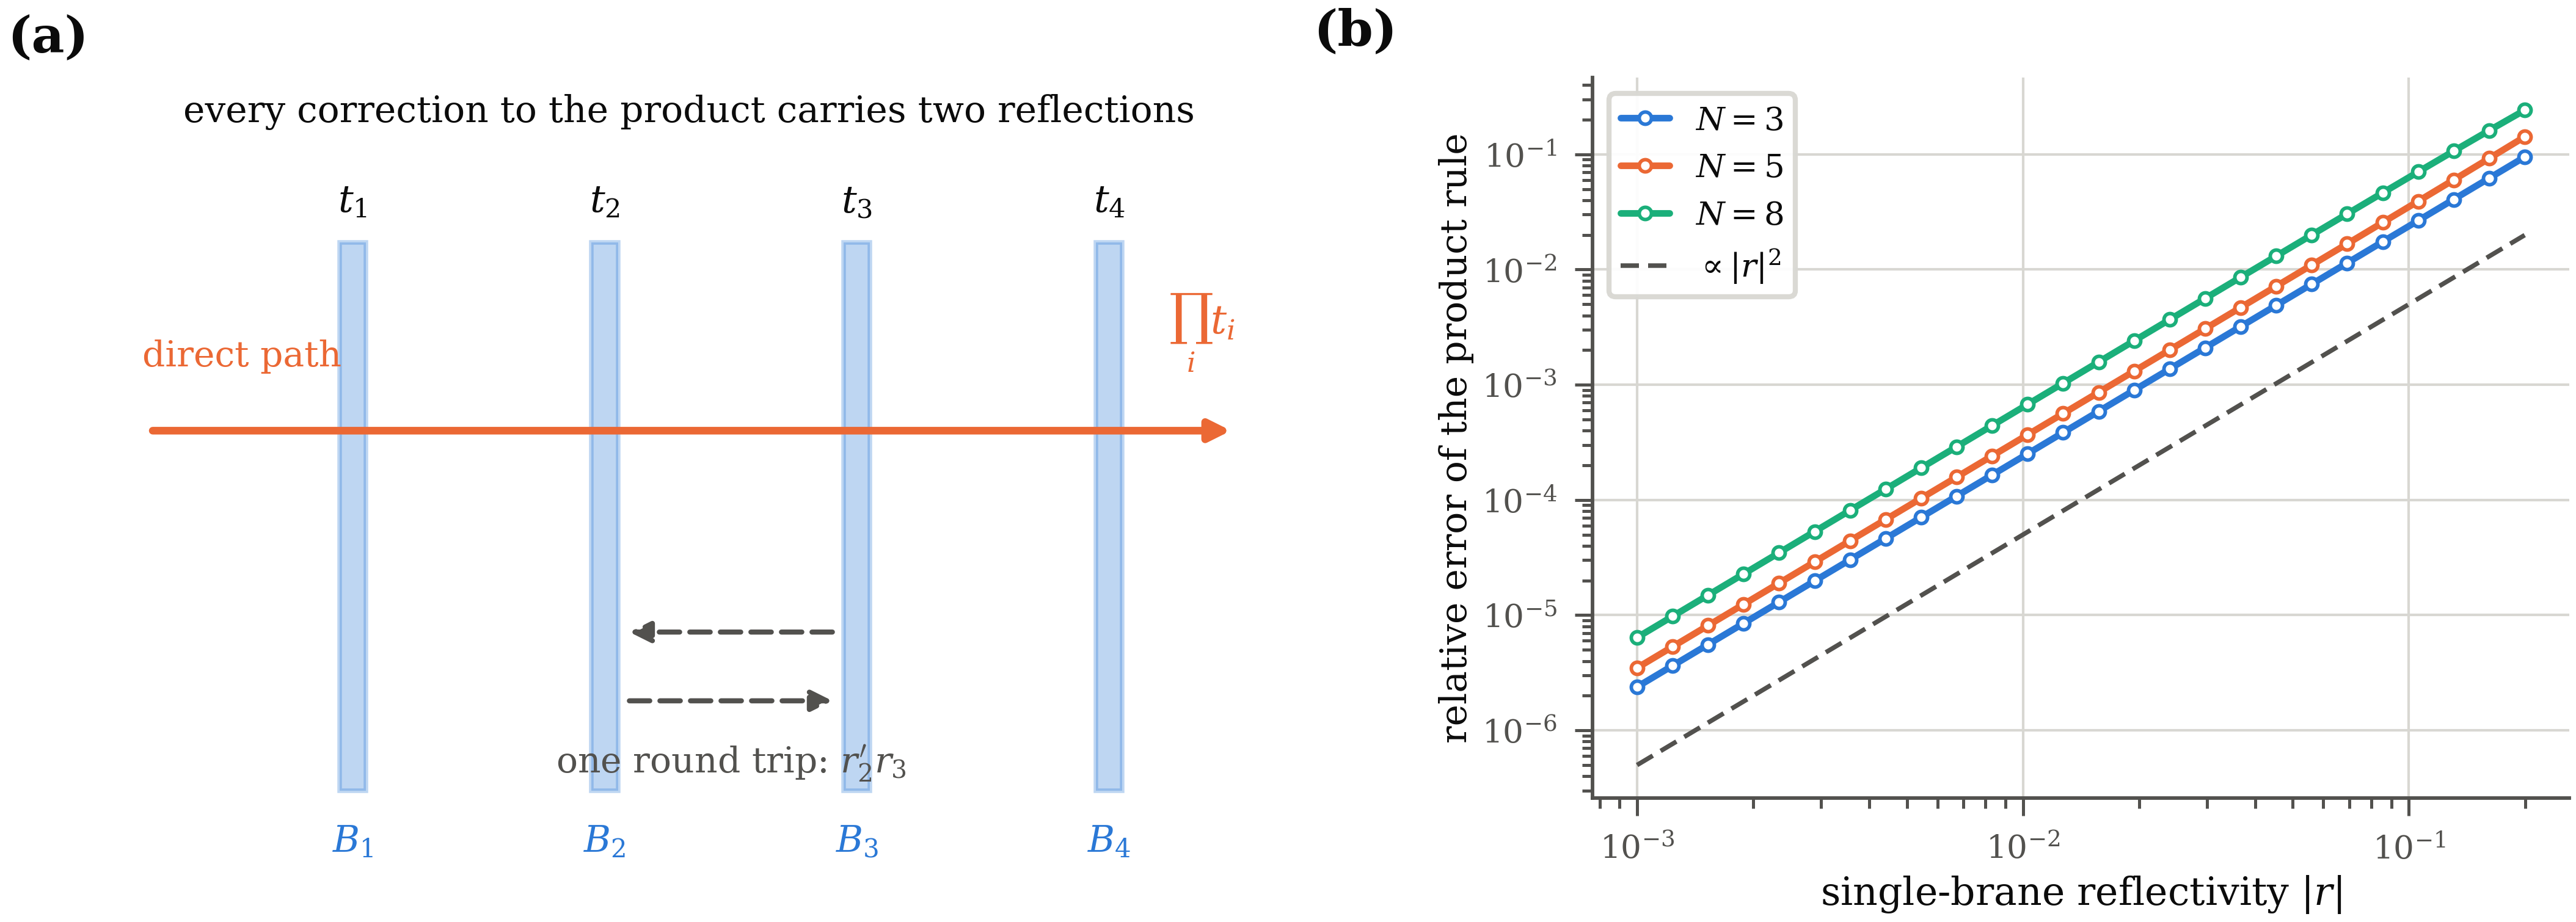
\includegraphics[width=\textwidth]{figs/fig07_transfer.png}
\caption{Lemma~\ref{lem:compose}. (a) A mode crossing a stack of branes. The direct path contributes the product of the single-brane transmission amplitudes, and every correction to that product contains a round trip, hence two reflection amplitudes. (b) The relative error of the product rule against the exact transfer-matrix result for a stack of $N$ identical branes, as a function of the single-brane reflectivity; the dashed guide is $|r|^2$. The error grows with the number of pairs, as \eqref{eq:product} requires.}
\label{fig:transfer}
\end{figure*}

\begin{hypothesis}[dilute independent branes]
\label{hyp:mult}
The reflection amplitudes are small enough that $\sum_{i<j}|r_i||r_j|\ll1$, so that \eqref{eq:product} may be used with $\mathcal E$ dropped, and the derivative expansion \eqref{eq:derivexp} is truncated at its first nontrivial order.
\end{hypothesis}

Under Hypothesis~\ref{hyp:mult} the dressed kinetic operator is $p^2a_\cB(p^2)$ with

\begin{equation}
\label{eq:cluster-sum}
a_\cB(z)=\prod_{i=1}^{N}\Bigl(1+\frac{w_iz}{M^2}\Bigr)
=\sum_{S\subseteq\{1,\dots,N\}}\ \prod_{i\in S}\frac{w_iz}{M^2},
\end{equation}
the sum on the right running over all subsets, including the empty one, which contributes $1$.

Equation \eqref{eq:cluster-sum} says that the $K$-cluster $B_S$ contributes the product of the weights of the branes meeting along it, times $z^K$, so that a $K$-fold intersection carries $K$ extra derivative pairs. The number of terms in the sum is the number of strata, which for the coordinate arrangement of Proposition~\ref{prop:census} is $\sum_K\binom{D}{K}=2^D$, and the $K$-th group of terms is the $K$-cluster count $\binom DK$. This is the cluster expansion of the earlier proposal \cite{Bhattacharjee2025brane}, with the unspecified coefficients of that proposal replaced by explicit products of weights.

The alternative is worth writing down. If the branes contributed additively, each supplying a term $w_iz/M^2$ to the kinetic operator instead of a factor $1+w_iz/M^2$, the form factor would be $1+z\sum_iw_i/M^2$, a polynomial of degree one whatever the number of branes. By Theorem~\ref{thm:sumrule} that single zero carries residue exactly $-1$, so an additive arrangement of any size reproduces the pole content of curvature-squared gravity and nothing else. The higher strata would be invisible. Only multiplicativity lets the intersections contribute at all, and only multiplicativity makes the degree grow with $N$, which the power counting of Sec.~\ref{sec:power} requires. Both readings are covered by the sum rule, and neither escapes it.

\begin{proposition}[deterministic arrangements]
\label{prop:poly}
The two expressions in \eqref{eq:cluster-sum} agree, and $a_\cB$ is a polynomial of degree $N'=\#\{i:w_i>0\}$ whose zeros lie at $z=-M^2/w_i$.
\end{proposition}

\begin{proof}
Expand the product. Choosing the second term of the $i$-th factor for every $i$ in a subset $S$, and the first term otherwise, produces the monomial indexed by $S$ once and only once, so the subsets index the terms of the sum. A factor with $w_i=0$ is $1$ and contributes no zero, and each factor with $w_i>0$ contributes the simple zero $z=-M^2/w_i$.
\end{proof}

\begin{remark}[the census reappears as the order of a zero]
\label{rem:euler-zero}
Take the coordinate arrangement of Proposition~\ref{prop:census} with all weights equal to $w$. The subset sum \eqref{eq:cluster-sum} then has $\binom DK$ identical terms at each $K$, so $a_\cB(z)=\sum_K\binom DK(wz/M^2)^K$, and at $z=-M^2/w$ this is $\sum_K(-1)^K\binom DK$. By \eqref{eq:census} that sum vanishes, which says that $a_\cB$ has a zero there, and Proposition~\ref{prop:poly} identifies it as a zero of order $D$. The vanishing alternating sum of the census and the degenerate pole of the propagator are one statement, read from either end of the construction.
\end{remark}

\subsection{The Poisson gas}

Now let the arrangement be random. A \emph{brane gas} is a Poisson point process $\Pi$ on a measurable space $\mathcal S$ of branes (positions, orientations, and any internal labels) with a finite intensity measure $\Lambda$; the number of branes in a measurable set $A\subseteq\mathcal S$ is Poisson with mean $\Lambda(A)$, and the counts in disjoint sets are independent \cite{Kingman1993,LastPenrose2017}. The weight of a brane is a measurable function $w:\mathcal S\to[0,\infty)$, bounded.

\begin{theorem}[the gas exponentiates]
\label{thm:poisson}
Let $\Pi$ be a brane gas with intensity $\Lambda$ and weights $w$. Then for every $z\in\bC$
\begin{equation}
\label{eq:pgfl}
\bE\Bigl[\prod_{x\in\Pi}\Bigl(1+\frac{w(x)z}{M^2}\Bigr)\Bigr]=\exp\Bigl(\frac{z}{M^2}\int_{\mathcal S}w\,\dd\Lambda\Bigr),
\end{equation}
and the expected number of $K$-clusters weighted by their products is $\frac{1}{K!}\bigl(\int w\,\dd\Lambda\bigr)^K$. More generally, if each brane contributes a factor $1+u(x,z)$ with $u(x,\cdot)$ entire for every $x$ and $\sup_x|u(x,z)|$ bounded on compact sets, then
\begin{equation}
\label{eq:pgfl-general}
\bE\Bigl[\prod_{x\in\Pi}\bigl(1+u(x,z)\bigr)\Bigr]=e^{H(z)},\quad H(z)=\int_{\mathcal S}u(x,z)\,\dd\Lambda(x),
\end{equation}
with $H$ entire and $H(0)=0$ when $u(x,0)=0$.
\end{theorem}

\begin{proof}
Write $\lambda=\Lambda(\mathcal S)<\infty$. A Poisson process with finite intensity measure has the following description: the number $N$ of points is Poisson with mean $\lambda$, and given $N$ the points $X_1,\dots,X_N$ are independent with the common law $\Lambda/\lambda$ \cite[Chapter~3]{LastPenrose2017}. For bounded $u(\cdot,z)$ the factors are bounded and
\begin{align*}
\bE\Bigl[\prod_{k=1}^{N}\bigl(1+u(X_k,z)\bigr)\Bigr]
&=\sum_{N\ge0}\frac{e^{-\lambda}\lambda^N}{N!}\Bigl(1+\frac1\lambda\int u\,\dd\Lambda\Bigr)^{N}\\
&=\exp\Bigl(\int_{\mathcal S}u(x,z)\,\dd\Lambda(x)\Bigr),
\end{align*}
which is \eqref{eq:pgfl-general}, and \eqref{eq:pgfl} is the case $u=wz/M^2$. The function $H$ is continuous in $z$ by dominated convergence, and its integral over every closed triangle vanishes by Fubini and Cauchy's theorem applied to each $u(x,\cdot)$, so $H$ is entire by Morera's theorem; $H(0)=\int u(x,0)\,\dd\Lambda=0$ when $u(x,0)=0$. For the cluster count, expand the product over the $N$ points: the $K$-subsets contribute $\sum_{|S|=K}\prod_{k\in S}w(X_k)z/M^2$, whose expectation is
\begin{align*}
&\Bigl(\frac{z}{M^2}\Bigr)^{K}\sum_{N\ge K}\frac{e^{-\lambda}\lambda^N}{N!}\binom NK\Bigl(\frac1\lambda\int w\,\dd\Lambda\Bigr)^{K}\\
&\qquad=\frac{1}{K!}\Bigl(\frac{z}{M^2}\int w\,\dd\Lambda\Bigr)^{K},
\end{align*}
the $K$-th term of the exponential series. Equivalently, the $K$-th factorial moment measure of a Poisson process is $\Lambda^{\otimes K}$ \cite[Chapter~4]{LastPenrose2017}, and the sum over unordered $K$-subsets is the integral against $\Lambda^{\otimes K}/K!$.
\end{proof}

\begin{remark}[linked clusters]
Equation \eqref{eq:pgfl} is the linked-cluster theorem in its simplest form. The full sum over strata, the left side, is the exponential of the sum over single branes, the exponent. In a gas the connected part of the cluster expansion is one brane deep, and every higher cluster is a product of independent factors, which is why the $1/K!$ of the exponential series is exactly the $1/K!$ of unordered $K$-subsets. Two kinds of truncation behave quite differently here. Cutting the sum over strata at $K\le N_0$ leaves a polynomial, which falls under Proposition~\ref{prop:poly}; cutting the exponent $H$ at any finite order leaves $e^{H}$ zero-free. The gas must therefore be resummed on the exponent and not on the sum.
\end{remark}

\subsection{Annealed and quenched form factors}
\label{sec:annealed}

The exponential of Theorem~\ref{thm:poisson} is an average, and which average it is decides what the rest of the paper is about. We set the two readings side by side here, because every later statement inherits the difference.

\begin{remark}[the average does not commute with inversion]
\label{rem:annealed}
The right side of \eqref{eq:pgfl} is the mean of the kinetic operator, not the mean of the propagator:
\begin{equation}
\label{eq:noncommute}
\bE\Bigl[\frac{1}{z\,a_\Pi(z)}\Bigr]\ \neq\ \frac{1}{z\,\bE[a_\Pi(z)]} .
\end{equation}
The left side is the quenched propagator, obtained by averaging observables over frozen realizations of the gas; the right side is the annealed one, obtained by averaging the action before inverting. Jensen's inequality already shows that the two differ, and \eqref{eq:noncommute} is strict whenever $a_\Pi$ is not deterministic.
\end{remark}

In the annealed regime the branes fluctuate quickly compared with the graviton, so that integrating out the brane sector leaves the metric coupled to the mean operator. The effective quadratic action then carries $\bE[a_\Pi]=e^{H}$, which has no zeros, and the conclusions of Secs.~\ref{sec:poles} to \ref{sec:gaussian} apply as stated: one pole, positive residue, a regular potential.

In the quenched regime the arrangement is frozen on the time scale of the experiment. Each realization carries the polynomial of Proposition~\ref{prop:poly} with its full complement of poles, and Theorem~\ref{thm:sumrule} assigns residues summing to $-1$ to every one of them. Averaging over realizations does not help, because it is an average of propagators each of which already contains the negative residues. No cancellation between realizations can produce a positive spectral density from a family of measures that each fail to have one.

The control parameter is the ratio of the correlation time of the gas to the inverse momentum at which the graviton is probed, and the annealed description requires it to be small. This is the same dilute, weakly reflecting regime that justified Hypothesis~\ref{hyp:mult}, so the two approximations of the model succeed or fail together. Making the ghost-free conclusion conditional on the annealed description therefore does not weaken it. It states the regime in which the model is defined at all. Figure~\ref{fig:annealed} puts the two side by side for a five-brane gas: the frozen realizations each spike at their own poles and each carry residues summing to $-1$, while the annealed propagator has no massive pole at all.

\begin{figure*}[t]
\centering
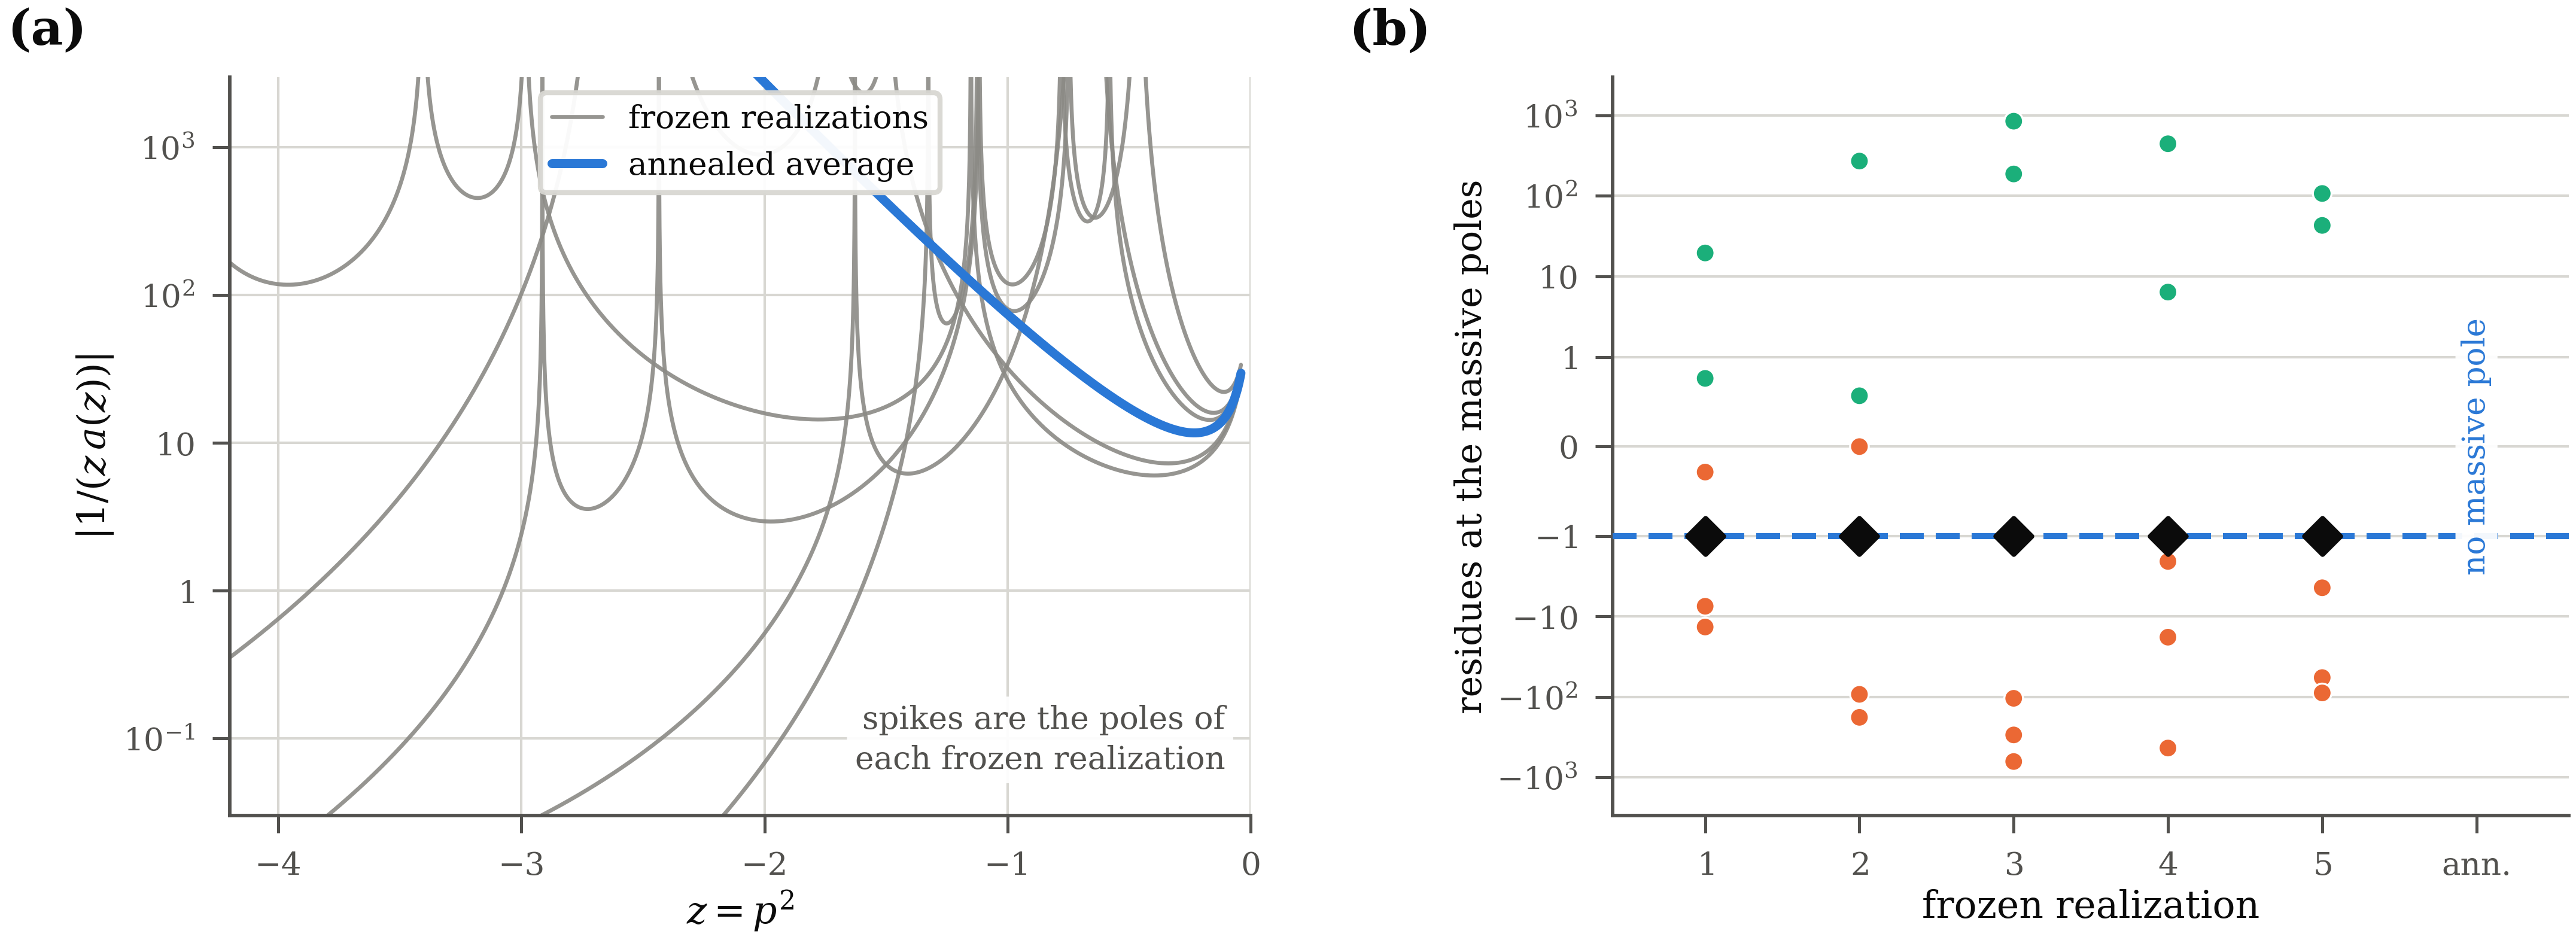
\includegraphics[width=\textwidth]{figs/fig08_annealed.png}
\caption{Annealed against quenched, for a five-brane gas. (a) The modulus of the spin-two propagator along the negative real axis for five frozen realizations, each spiking at its own poles, against the annealed propagator built from the averaged kinetic operator. The annealed curve is finite at every $z\neq0$ and simply leaves the plotted range; it has no pole. (b) The residues at the massive poles of each realization, which scatter over four decades, and their total, which is $-1$ in every case by Theorem~\ref{thm:sumrule}. The annealed form factor has no massive pole and so no budget to balance.}
\label{fig:annealed}
\end{figure*}


\section{The dressed graviton}
\label{sec:propagator}

\subsection{Action and propagator}

Expand $g_{\mu\nu}=\eta_{\mu\nu}+\kappa h_{\mu\nu}$, $\kappa^2=32\pi G$, in Euclidean signature, and let $\theta_{\mu\nu}=\eta_{\mu\nu}-p_\mu p_\nu/p^2$ and $\omega_{\mu\nu}=p_\mu p_\nu/p^2$. The spin projectors of Barnes and Rivers \cite{Rivers1964,VanNieuwenhuizen1973} on symmetric rank-two tensors are
\begin{align}
\Pt_{\mu\nu\alpha\beta}&=\tfrac12(\theta_{\mu\alpha}\theta_{\nu\beta}+\theta_{\mu\beta}\theta_{\nu\alpha})-\tfrac1{D-1}\theta_{\mu\nu}\theta_{\alpha\beta},\notag\\
P^{(1)}_{\mu\nu\alpha\beta}&=\tfrac12(\theta_{\mu\alpha}\omega_{\nu\beta}+\theta_{\mu\beta}\omega_{\nu\alpha}+\omega_{\mu\alpha}\theta_{\nu\beta}+\omega_{\mu\beta}\theta_{\nu\alpha}),\label{eq:projectors}\\
\Ps_{s}&=\tfrac1{D-1}\theta_{\mu\nu}\theta_{\alpha\beta},\qquad
\Ps_{w}=\omega_{\mu\nu}\omega_{\alpha\beta}.\notag
\end{align}

\begin{lemma}
\label{lem:projectors}
$\Pt+P^{(1)}+\Ps_s+\Ps_w=\mathbf 1$, the four operators are idempotent and mutually orthogonal, $p^\mu\Pt_{\mu\nu\alpha\beta}=0$, and $\Pt$ has trace $\tfrac12D(D+1)-D-1$, which is $5$ in $D=4$.
\end{lemma}

\begin{proof}
$\theta$ and $\omega$ are complementary orthogonal projectors on vectors, $\theta+\omega=\eta$, $\theta^2=\theta$, $\omega^2=\omega$, $\theta\omega=0$; the four tensors are the symmetrized products of these with the trace part separated, and the relations follow by substitution. Transversality is $p^\mu\theta_{\mu\nu}=0$. The trace of $\Pt$ is the dimension of the space of symmetric transverse traceless tensors.
\end{proof}

With a form factor $a(p^2)$ on the spin-two part and $b(p^2)$ on the spin-zero part, both normalized to $1$ at $p^2=0$, the gauge-invariant part of the quadratic action is
\begin{equation}
\label{eq:quad}
S^{(2)}=\frac12\!\int\!\frac{\dd^Dp}{(2\pi)^D}\,h(-p)\Bigl[p^2a\,\Pt-\frac{p^2b}{D-2}\Ps_s\Bigr]h(p),
\end{equation}
and its inverse on the gauge-invariant subspace is the propagator
\begin{equation}
\label{eq:propagator}
\Pi(p)=\frac{\Pt}{p^2a(p^2)}-\frac{(D-2)^{-1}\Ps_s}{p^2b(p^2)} .
\end{equation}
The infrared limit of \eqref{eq:propagator} is the Einstein propagator, and $b$ plays no part below, and $a$ carries the dressing the brane gas supplies; the form factor on the spin-zero part is fixed by requiring that the local part of the action be Einstein--Hilbert, which gives $b=a$ in the standard construction \cite{BGKM2012}.

\begin{proposition}[Ward identity]
\label{prop:ward}
$p^\mu\Pi_{\mu\nu\alpha\beta}(p)\big|_{\text{spin-}2}=0$ identically in $p$ and for every form factor $a$.
\end{proposition}

\begin{proof}
The form factor multiplies $\Pt$ by a scalar and cannot spoil $p^\mu\Pt_{\mu\nu\alpha\beta}=0$.
\end{proof}

The full Slavnov--Taylor identity of the gauge-fixed theory, and the statement that the counterterms it admits are local diffeomorphism-invariant functionals, follow from the general cohomological analysis of \cite{BarnichBrandtHenneaux2000} once the power counting of Sec.~\ref{sec:power} bounds the dimension of the divergences; we use this only in Corollary~\ref{cor:counterterms} and do not reproduce the argument.

\section{Poles and residues}
\label{sec:poles}

\begin{theorem}[dichotomy]
\label{thm:dichotomy}
Let $a$ be a nonconstant entire function with $a(0)=1$ and let $\Pi_2(z)=1/(za(z))$ be the spin-two propagator as a function of $z=p^2$. Exactly one of the following holds.
\begin{enumerate}[label=\textup{(\alph*)},leftmargin=2.2em,itemsep=0.1em]
\item $a$ has a zero. Then $\Pi_2$ has at least one pole other than $z=0$, and if $a$ is a polynomial of degree $N$, exactly $N$ counted with multiplicity.
\item $a$ has no zero. Then $a=e^{H}$ for an entire $H$ with $H(0)=0$, and $\Pi_2$ has exactly one pole, a simple pole at $z=0$ with residue $+1$; if $a$ has finite order $\rho$ then $H$ is a polynomial of degree $\lfloor\rho\rfloor$.
\end{enumerate}
\end{theorem}

\begin{proof}
(a) A zero $z_0$ of the entire function $a$ is isolated and of finite order, and $z_0\ne0$ because $a(0)=1$, so $1/(za(z))$ has a pole at $z_0$. For a polynomial the number of zeros with multiplicity is the degree.

(b) On the simply connected domain $\bC$ a nonvanishing entire function has a single-valued entire logarithm $H$, normalized by $H(0)=\log a(0)=0$, and $a=e^{H}$. Then $\Pi_2=e^{-H(z)}/z$ has a simple pole at $0$ with residue $e^{-H(0)}=1$ and no other singularity, $e^{-H}$ being entire. If $a$ has finite order $\rho$, Hadamard's factorization theorem \cite{Hadamard1893}, \cite[Chapter~XI]{Conway1978} says that a zero-free entire function of order $\rho$ is $e^{P}$ with $P$ a polynomial of degree at most $\lfloor\rho\rfloor$, and since the order of $e^{P}$ is $\deg P$ the degree is exactly $\lfloor\rho\rfloor$.
\end{proof}

\begin{theorem}[sum rule]
\label{thm:sumrule}
Let $a$ be a polynomial of degree $N\ge1$ with $a(0)=1$, and let $z_1,\dots,z_r$ be its distinct zeros. Then the residues of $\Pi_2=1/(za(z))$ satisfy
\begin{equation}
\label{eq:sumrule}
\Res_{z=0}\Pi_2=1,\qquad \sum_{i=1}^{r}\Res_{z=z_i}\Pi_2=-1 .
\end{equation}
If the zeros are simple, real and negative, $z_i=-M_i^2$ with $0<M_1^2<\cdots<M_N^2$, then
\begin{equation}
\label{eq:residues}
\Res_{z=-M_i^2}\Pi_2=r_i=\frac{-1}{\prod_{j\neq i}\bigl(1-M_i^2/M_j^2\bigr)},
\end{equation}
the $r_i$ alternate in sign and $r_1<0$. In general, at least one massive residue has negative real part, and the massive residues cannot all be positive real numbers.
\end{theorem}

\begin{proof}
$\Pi_2$ is a rational function that decays like $z^{-N-1}$ at infinity, so the integral of $\Pi_2$ over a circle of radius $R$ tends to zero as $R\to\infty$; by the residue theorem the sum of all residues vanishes, and the residue at $0$ is $1/a(0)=1$, which gives \eqref{eq:sumrule}. For simple zeros, $\Res_{z_i}\Pi_2=1/(z_ia'(z_i))$; with $a(z)=\prod_j(1+z/M_j^2)$ this is $1/\bigl(-M_i^2\cdot M_i^{-2}\prod_{j\ne i}(1-M_i^2/M_j^2)\bigr)$, which is \eqref{eq:residues}. In the product, the factor with index $j$ is positive for $M_j^2>M_i^2$ and negative for $M_j^2<M_i^2$, so the product has sign $(-1)^{i-1}$ and $r_i$ has sign $(-1)^i$. The last statements follow from \eqref{eq:sumrule}: the real parts of the massive residues sum to $-1$, so one of them is negative, and positive reals cannot sum to $-1$.
\end{proof}

\begin{corollary}
\label{cor:ghostfree}
Within the class of propagators \eqref{eq:propagator} with $a$ entire, the spin-two sector has a single pole of positive residue if and only if $a=e^{H}$ with $H$ entire and $H(0)=0$. A deterministic arrangement of $N\ge1$ weighted branes under Hypothesis~\ref{hyp:mult} always has $N$ extra poles with residues summing to $-1$; a Poisson gas has none.
\end{corollary}

\begin{proof}
Theorem~\ref{thm:dichotomy} gives the equivalence, Proposition~\ref{prop:poly} and Theorem~\ref{thm:sumrule} the first statement, and Theorem~\ref{thm:poisson} the second.
\end{proof}

The dichotomy is visible in the surface $\log|a|$ over the complex plane, drawn in Fig.~\ref{fig:formfactor}: a deterministic arrangement digs one logarithmic pit at each zero, and the Poisson average has none.

\begin{figure*}[t]
\centering
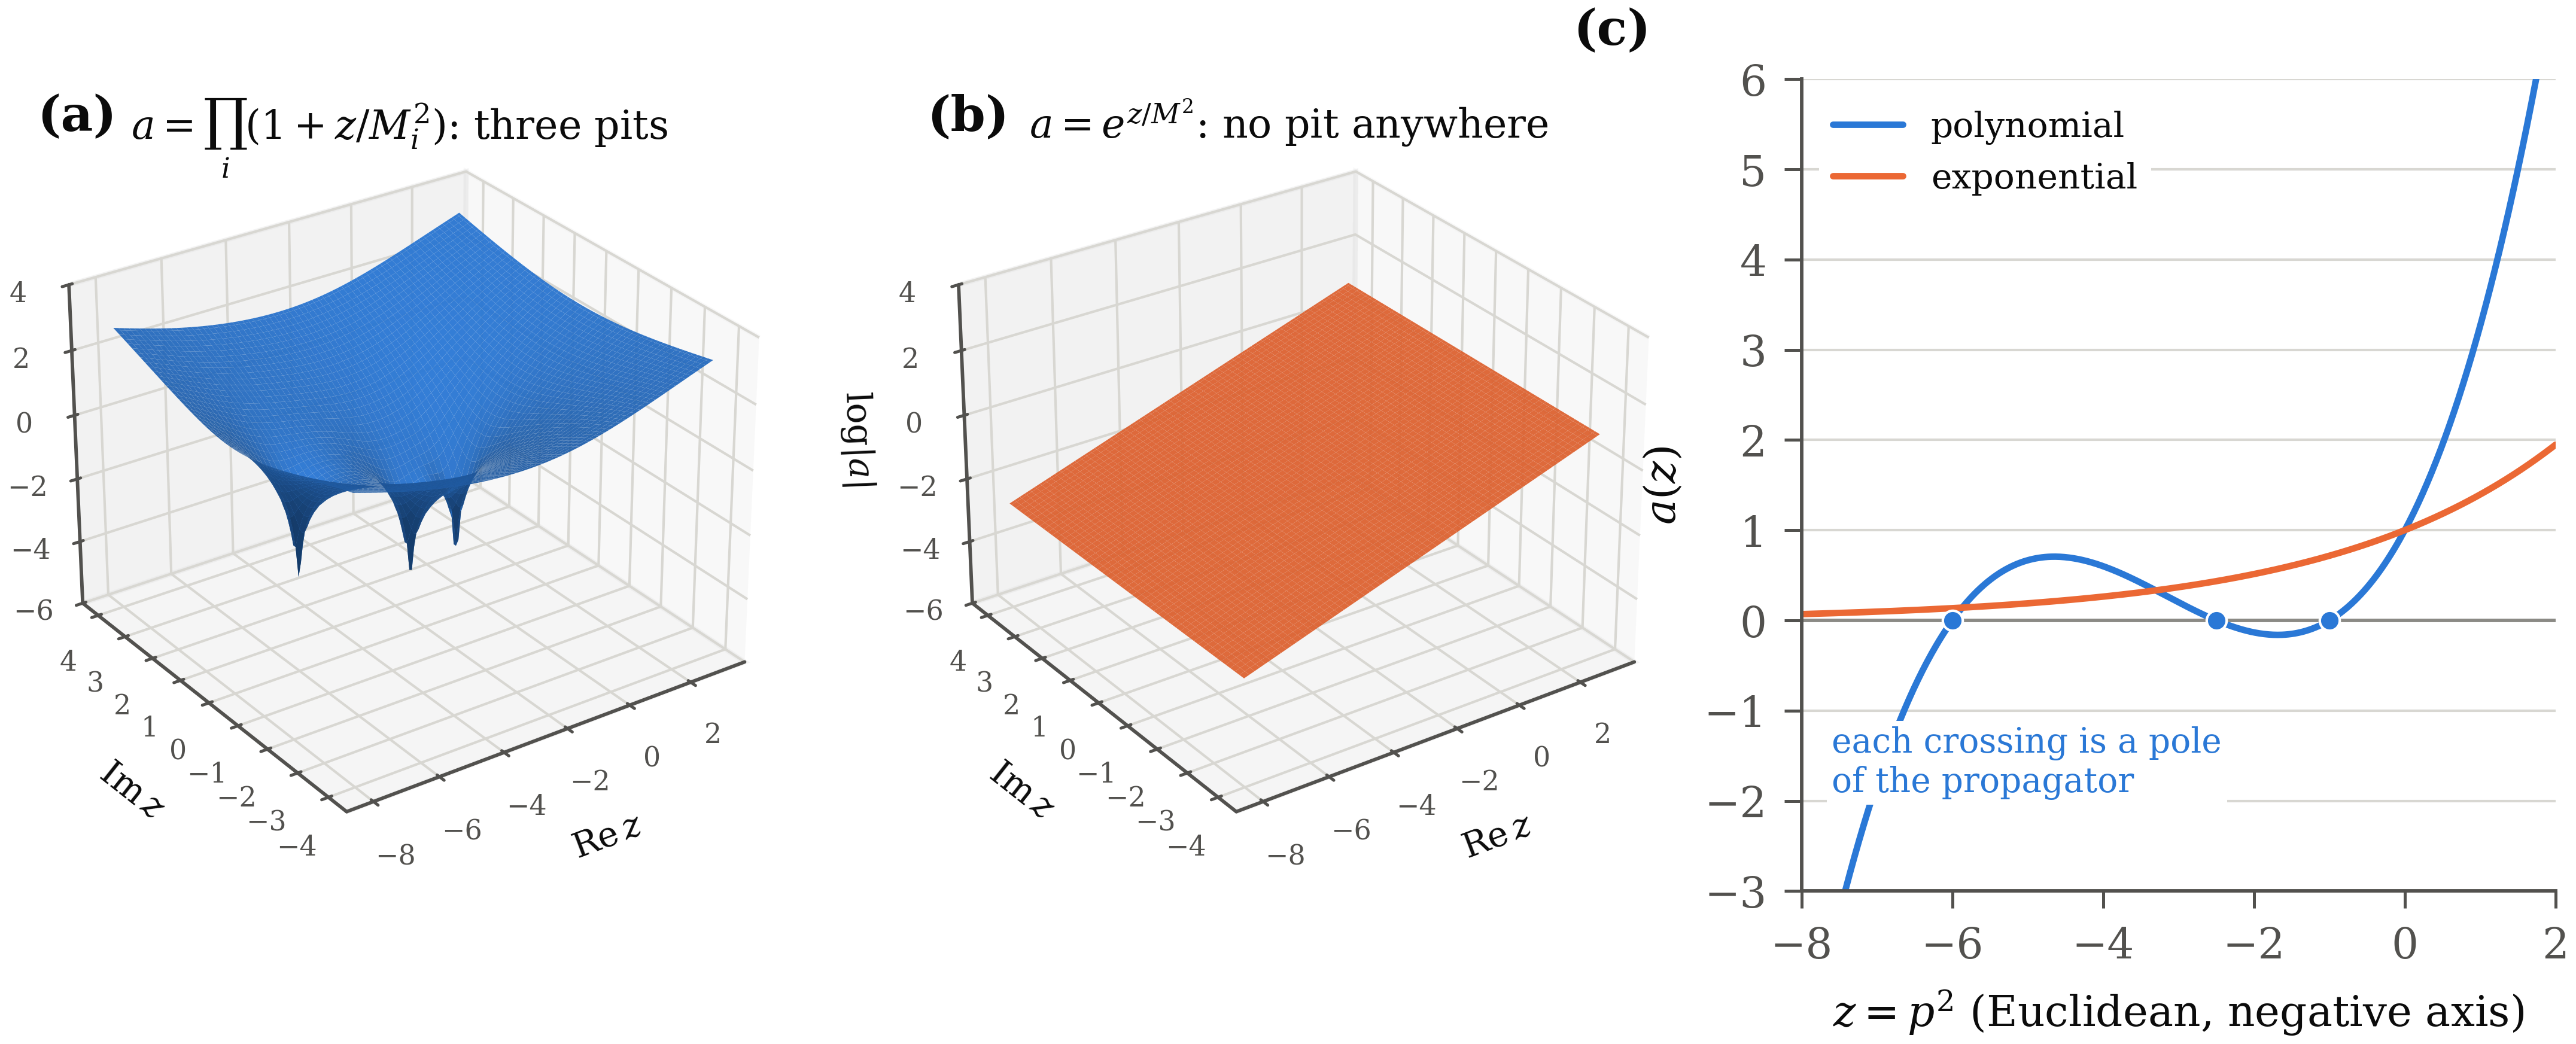
\includegraphics[width=\textwidth]{figs/fig03_formfactor.png}
\caption{(a) $\log|a(z)|$ over the complex $z=p^2$ plane for the arrangement of three branes with $a(z)=(1+z)(1+z/2.5)(1+z/6)$: three logarithmic pits at the zeros, each a pole of the propagator. (b) The same for the Poisson average $a(z)=e^{z/3}$: a plane, no pit anywhere. (c) Along the negative real axis the polynomial crosses zero three times and the exponential never does; the crossings are the masses of the extra poles.}
\label{fig:formfactor}
\end{figure*}

\begin{remark}[why this is not a choice of scheme]
The number and the residues of the poles of $\Pi_2$ are properties of the analytic function $a$. No field redefinition, choice of gauge or subtraction removes a zero of an entire function, and the residues \eqref{eq:residues} are computed from $a$ alone; the sum rule \eqref{eq:sumrule} is the residue theorem and no more. The statement is therefore not a perturbative one.

Two strands of the literature are worth placing against it. Shapiro \cite{Shapiro2015} counts the ghosts of polynomial form factors case by case and finds that they are always present; \eqref{eq:sumrule} gives the reason in a single line and fixes the total instead of the count, so it applies to degenerate zeros, to complex conjugate pairs, and to any normalization of $a$ with $a(0)=1$. Anselmi \cite{Anselmi2017,AnselmiPiva2017} proposes that complex conjugate pairs be quantized as fake degrees of freedom, removed from the physical spectrum by a modified prescription. The sum rule does not decide that proposal, but it does constrain it: whatever prescription is adopted, the residues at the poles other than $z=0$ still add to $-1$, so the negative weight is redistributed rather than removed, and a prescription that claims to dispose of it must say which pole absorbs it. The polynomial-derivative theories to which both discussions apply are the ones classified by Asorey, Lopez and Shapiro \cite{AsoreyLopezShapiro1997}, whose power counting is the $n\ge1$ case of Theorem~\ref{thm:power}.
\end{remark}

\begin{proposition}[curvature-squared gravity]
\label{prop:stelle}
Stelle's theory \cite{Stelle1977} has $a(z)=1+z/M^2$, so
\begin{equation}
\label{eq:stelle}
\frac{1}{z(1+z/M^2)}=\frac1z-\frac{1}{z+M^2},
\end{equation}
a massless graviton of residue $+1$ and a massive spin-two excitation of residue exactly $-1$: the sum rule with a single term. The classical face of the negative residue is the Ostrogradsky instability of the higher-derivative action \cite{Ostrogradsky1850,Woodard2015}.
\end{proposition}

Figure~\ref{fig:residues}(a) shows the alternation and the total for three arrangements with real masses; the other two panels belong to the power counting of Sec.~\ref{sec:power}.

\begin{figure*}[t]
\centering
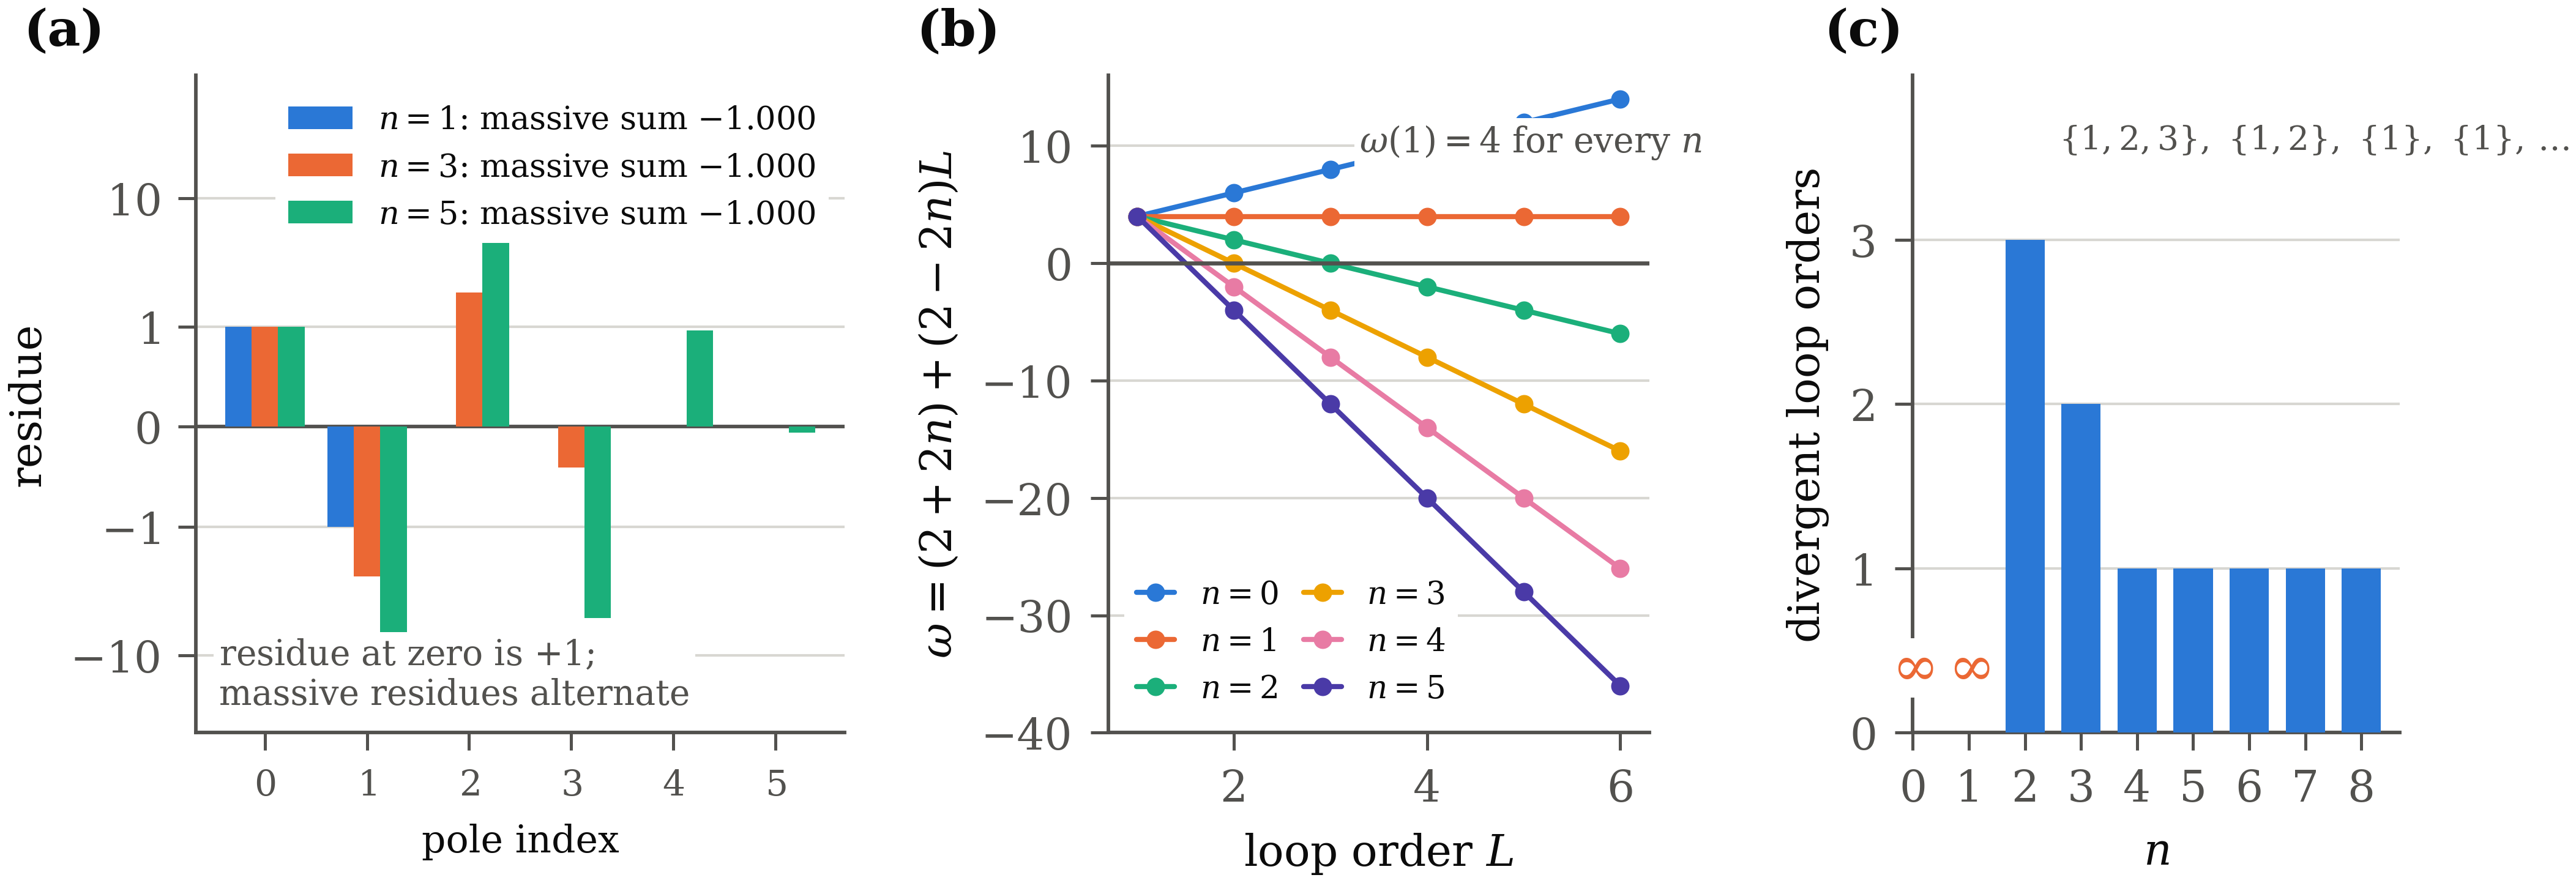
\includegraphics[width=\textwidth]{figs/fig04_residues.png}
\caption{(a) Residues of $1/(za(z))$ at the poles of the propagator for three deterministic arrangements with real masses, ordered by mass: the residue at zero is $+1$, the massive residues alternate starting negative, and in every case they sum to $-1$ (Theorem~\ref{thm:sumrule}). The vertical scale is linear within one unit of zero and logarithmic outside it, so that the five-mass case, whose residues run from $-7.0$ to $+10.2$, fits beside the others. (b) The superficial degree of divergence $\omega(L)$ in four dimensions for $n=0,\dots,5$ (Theorem~\ref{thm:power}); $\omega(1)=4$ for every $n$. (c) The number of divergent loop orders: infinite for $n\le1$, then $3$, $2$, and $1$ for every $n\ge4$.}
\label{fig:residues}
\end{figure*}

\section{Power counting}
\label{sec:power}

The degree of divergence of a graph depends on how the form factor grows. Two classes are relevant. If $a(p^2)$ grows like a power, $a(p^2)\sim p^{2n}$ as $p^2\to\infty$ in the Euclidean region, the propagator falls as $p^{-2-2n}$ and, by diffeomorphism invariance, which ties the vertex form factors to the propagator, the vertices grow as $p^{2+2n}$; this is the situation for the form factors of Tomboulis and Modesto \cite{Tomboulis1997,Modesto2012,ModestoRachwal2014}, which are constructed precisely so that $e^{H}$ has polynomial asymptotics along the real axis while $H$ remains entire. If instead $a=e^{z/M^2}$ exactly, the propagator is exponentially damped and the vertices exponentially enhanced, and the counting below does not apply; the ultraviolet behavior of loops is then a subtler matter \cite{Talaganis2015}.

\begin{hypothesis}[polynomial growth]
\label{hyp:growth}
$a$ is entire with $a(0)=1$ and $|a(p^2)|\sim c\,p^{2n}$ as $p^2\to+\infty$, and the vertex form factors grow as $p^{2+2n}$.
\end{hypothesis}

\begin{theorem}
\label{thm:power}
Under Hypothesis~\ref{hyp:growth}, for every connected graph in $D$ spacetime dimensions with $V$ vertices, $I$ internal lines and $L=I-V+1$ loops, the superficial degree of divergence is
\begin{equation}
\label{eq:omega}
\omega=DL-(2+2n)I+(2+2n)V=(2+2n)+(D-2-2n)L,
\end{equation}
independent of the topology of the graph beyond $L$. In $D=4$, $\omega<0$ if and only if $L>(n+1)/(n-1)$ when $n\ge2$, and $\omega\ge0$ for every $L$ when $n\le1$; the loop orders at which a graph can diverge are all $L$ for $n\le1$, $\{1,2,3\}$ for $n=2$, $\{1,2\}$ for $n=3$ and $\{1\}$ for every $n\ge4$. In general dimension $D$ only one-loop graphs can diverge exactly when $n\ge D$, and $\omega(L=1)=D$ for every $n$.
\end{theorem}

\begin{proof}
Each loop integration contributes $D$ powers of momentum, each internal line $-(2+2n)$ and each vertex $+(2+2n)$, so $\omega=DL-(2+2n)I+(2+2n)V$, and substituting $I=L+V-1$ removes $V$. In $D=4$, $\omega=(2+2n)+(2-2n)L<0$ is $(2n-2)L>2n+2$, that is $L>(n+1)/(n-1)$ for $n\ge2$; for $n=1$ the left side is $0$ and $\omega=4$, for $n=0$ $\omega=2+2L>0$. The thresholds are $3$ for $n=2$, $2$ for $n=3$, and $(n+1)/(n-1)<2$ for $n\ge4$. In dimension $D$ the function $L\mapsto\omega$ is affine with slope $D-2-2n$, so every $L\ge2$ is finite exactly when $\omega(2)=2D-2-2n<0$, that is $n\ge D$; and $\omega(1)=D$ from \eqref{eq:omega}.
\end{proof}

\begin{corollary}
\label{cor:counterterms}
Under Hypothesis~\ref{hyp:growth} with $n\ge4$ in $D=4$, the only divergent graphs are one-loop graphs, their divergences are local functionals of dimension at most four, and by the cohomological classification of \cite{BarnichBrandtHenneaux2000} they are diffeomorphism-invariant: linear combinations of $R^2$, $R_{\mu\nu}R^{\mu\nu}$, the Gauss--Bonnet density and a cosmological term, with coefficients that are polynomial in finitely many Taylor coefficients of $H$.
\end{corollary}

\begin{proof}
The loop count is Theorem~\ref{thm:power}. A superficially divergent one-loop graph with $\omega\le4$ has a divergent part polynomial in external momenta of degree at most four, hence local of dimension at most four; the invariant monomials of that dimension are the ones listed, up to the total derivative $\Box R$ and the Gauss--Bonnet identity eliminating the Riemann-squared term. The one-loop divergence is the logarithmically divergent part of $\tfrac12\operatorname{tr}\log\delta^2S$, given by the second heat-kernel coefficient of the fluctuation operator \cite{Vassilevich2003}, which depends on $H$ only through the finitely many Taylor coefficients that survive at that order.
\end{proof}

\begin{remark}
$\omega(L=1)=4$ for every $n$: no improvement of the propagator removes the one-loop divergence by counting alone, and its removal is a condition on finitely many coefficients of $H$, as in \cite{ModestoRachwal2014}. Whether these conditions are compatible with the requirement that $H$ be of the form produced by a gas, $H(z)=\int u(x,z)\,\dd\Lambda(x)$, depends on the family of couplings $u$ admitted, and is an open question of the model.
\end{remark}

\section{The Gaussian form factor}
\label{sec:gaussian}

The simplest zero-free form factor is the one produced by a gas with $u=wz/M^2$: after absorbing $\int w\,\dd\Lambda$ into $M$, $a(z)=e^{z/M^2}$ in Euclidean signature, that is $a(\Box)=e^{-\Box/M^2}$. This section collects what can be computed in closed form for it, starting with the loop integrals that Theorem~\ref{thm:power} excludes. The Newtonian potential below has appeared in the nonlocal gravity literature \cite{BGKM2012,EdholmKoshelevMazumdar2016,Buoninfante2018}; the $D$-dimensional propagator, its value at the origin and the threshold statement are given in the form we need, with proofs.

\subsection{Loop integrals in the parametric representation}

Hypothesis~\ref{hyp:growth} fails for the Gaussian, so the counting of Theorem~\ref{thm:power} says nothing about it. What takes its place is an exact statement about where the parametric integral lives. The observation is elementary, and it shows the Gaussian case to be better behaved than the counting would suggest.

\begin{lemma}[the Schwinger parameter is bounded below]
\label{lem:schwinger}
In Euclidean signature the dressed propagator of the Gaussian form factor admits the representation
\begin{equation}
\label{eq:schwinger}
\frac{e^{-k^2/M^2}}{k^2}=\int_{1/M^2}^{\infty}\dd s\;e^{-sk^2},
\end{equation}
so that the Schwinger parameter of every internal line is bounded below by $1/M^2$.
\end{lemma}

\begin{proof}
$\int_0^\infty\dd\alpha\,e^{-\alpha k^2}=1/k^2$ for $k^2>0$; substituting $s=\alpha+1/M^2$ shifts the lower limit and supplies the factor $e^{-k^2/M^2}$.
\end{proof}

\begin{theorem}[no ultraviolet divergence]
\label{thm:noUV}
Let $G$ be a connected Euclidean graph with $I$ internal lines, $V$ vertices and $L=I-V+1$ loops, every line carrying the dressed propagator $e^{-k^2/M^2}/k^2$ and every vertex a polynomial in the momenta. Then the loop integral of $G$ has the parametric representation
\begin{multline}
\label{eq:symanzik}
\mathcal I_G(p)=\frac{1}{(4\pi)^{DL/2}}\int_{[1/M^2,\infty)^I}\ \prod_{i=1}^{I}\dd s_i\\
\times\;\frac{\mathcal P_G(s,p)}{U_G(s)^{D/2}}\,
\exp\bigl(-F_G(s,p)/U_G(s)\bigr),
\end{multline}
with $U_G$ and $F_G$ the Symanzik polynomials of $G$ and $\mathcal P_G$ a polynomial in the external momenta and in $U_G^{-1}$. On this domain
\begin{equation}
\label{eq:Ubound}
U_G(s)\ \ge\ t(G)\,M^{-2L},
\end{equation}
where $t(G)$ is the number of spanning trees of $G$, and the integrand of \eqref{eq:symanzik} is bounded uniformly in $s$. The graph therefore has no ultraviolet divergence: the divergences of the undressed graph arise from the corner of parameter space in which the $s_i$ approach zero, and that corner has been removed. The behaviour at large $s_i$, and with it the infrared structure, is the same as for the undressed massless graph.
\end{theorem}

\begin{proof}
Write each line as \eqref{eq:schwinger} and carry out the $L$ Gaussian integrations over the loop momenta. This is the standard construction of the parametric representation \cite[Chapter~6]{Smirnov2006}: the result is \eqref{eq:symanzik} with
\begin{align*}
U_G(s)&=\sum_{T}\ \prod_{i\notin T}s_i,\\
F_G(s,p)&=\sum_{(T_1,T_2)}\ \Bigl(\prod_{i\notin T_1\cup T_2}s_i\Bigr)\,q(T_1,T_2)^2,
\end{align*}
the first sum running over the spanning trees $T$ of $G$ and the second over the two-forests, with $q(T_1,T_2)$ the momentum flowing between the two components. Vertex polynomials contribute the factor $\mathcal P_G$, which is polynomial in the external momenta and in $U_G^{-1}$ because each contraction of two loop momenta produces one inverse power of $U_G$.

Each monomial of $U_G$ is a product of exactly $L$ of the $s_i$ with coefficient one, so $U_G$ is nondecreasing in every $s_i$; evaluating at $s_i=M^{-2}$ for all $i$ gives \eqref{eq:Ubound}, the number of monomials being the number of spanning trees. For Euclidean external momenta $F_G\ge0$ and $U_G>0$, so the exponential in \eqref{eq:symanzik} is at most $1$. By \eqref{eq:Ubound} the factor $U_G^{-D/2}$ is bounded by $\bigl(t(G)\bigr)^{-D/2}M^{DL}$, and $\mathcal P_G$ is bounded on the domain for the same reason. The integrand is therefore bounded by a function of the external momenta alone, uniformly in $s$.

An ultraviolet divergence of the undressed graph is, in this representation, a non-integrable singularity produced as a subset of the $s_i$ tends to zero, where $U_G$ degenerates. No such limit exists on $[1/M^2,\infty)^I$. What remains is the region in which some $s_i$ grow without bound, which is the infrared region and is untouched by the form factor, since \eqref{eq:schwinger} modifies the integrand only near $s=0$.
\end{proof}

\begin{proposition}[the one-loop bubble]
\label{prop:bubble}
For the bubble, $I=2$, $L=1$, $U=s_1+s_2$ and $F=s_1s_2p^2$, so
\begin{multline}
\label{eq:bubble}
\mathcal I(p)=\frac{1}{(4\pi)^{D/2}}\int_{1/M^2}^{\infty}\dd s_1\int_{1/M^2}^{\infty}\dd s_2\\
\times\;\frac{1}{(s_1+s_2)^{D/2}}\,\exp\Bigl(-\frac{s_1s_2\,p^2}{s_1+s_2}\Bigr).
\end{multline}
This is finite for every $p$ when $D>4$, and at $p=0$ it evaluates to
\begin{equation}
\label{eq:bubble0}
\mathcal I(0)=\frac{2^{\,2-D/2}\,M^{D-4}}{(4\pi)^{D/2}\bigl(\tfrac D2-1\bigr)\bigl(\tfrac D2-2\bigr)} ,
\qquad D>4 .
\end{equation}
For $D=4$ the integral converges for $p^2>0$ and its $p\to0$ divergence is logarithmic and infrared, as it is for the undressed massless bubble.
\end{proposition}

\begin{proof}
The Symanzik polynomials of the bubble are as stated. At $p=0$ the exponential is $1$; put $u=s_1+s_2$, so that for $s_1,s_2\ge a$ the variable $u$ runs over $[2a,\infty)$ and the segment available to $s_1$ at fixed $u$ has length $u-2a$. Hence
\begin{align*}
\int_{a}^{\infty}\!\int_{a}^{\infty}\frac{\dd s_1\,\dd s_2}{(s_1+s_2)^{D/2}}
&=\int_{2a}^{\infty}\frac{u-2a}{u^{D/2}}\,\dd u\\
&=\frac{(2a)^{2-D/2}}{\bigl(\tfrac D2-1\bigr)\bigl(\tfrac D2-2\bigr)},
\end{align*}
both terms converging for $D>4$; setting $a=1/M^2$ gives \eqref{eq:bubble0}. For $D=4$ and $p^2>0$ the exponent $-s_1s_2p^2/(s_1+s_2)$ tends to $-\infty$ along every ray into the large-$s$ region except the two axial directions, along which the prefactor $(s_1+s_2)^{-2}$ is integrable, so the integral converges; as $p\to0$ the exponential ceases to damp and the logarithm appears, which is the infrared behaviour of the massless bubble and is independent of $M$.
\end{proof}

\begin{remark}[the vertices]
\label{rem:vertices}
Theorem~\ref{thm:noUV} assumes vertices polynomial in the momenta. In a gravitational theory built from $e^{-\Box/M^2}$ the vertices inherit the form factor and grow exponentially, and the cancellation between the damping of the propagators and the growth of the vertices makes the ultraviolet behavior of infinite-derivative gravity delicate; that regime is analysed in \cite{Talaganis2015}. The content of Theorem~\ref{thm:noUV} is that the difficulty is located entirely in the vertices: the propagators alone remove the ultraviolet corner of parameter space at every loop order, with the explicit bound \eqref{eq:Ubound}, and \eqref{eq:bubble0} is a closed-form instance. Any mechanism that keeps the vertices polynomially bounded therefore inherits a finite theory.
\end{remark}

Figure~\ref{fig:schwinger}(a) is the parameter plane of the bubble with the deleted corner shaded, and panel (b) follows the value of the integral out to large external momentum in three dimensions above four.

\begin{figure*}[t]
\centering
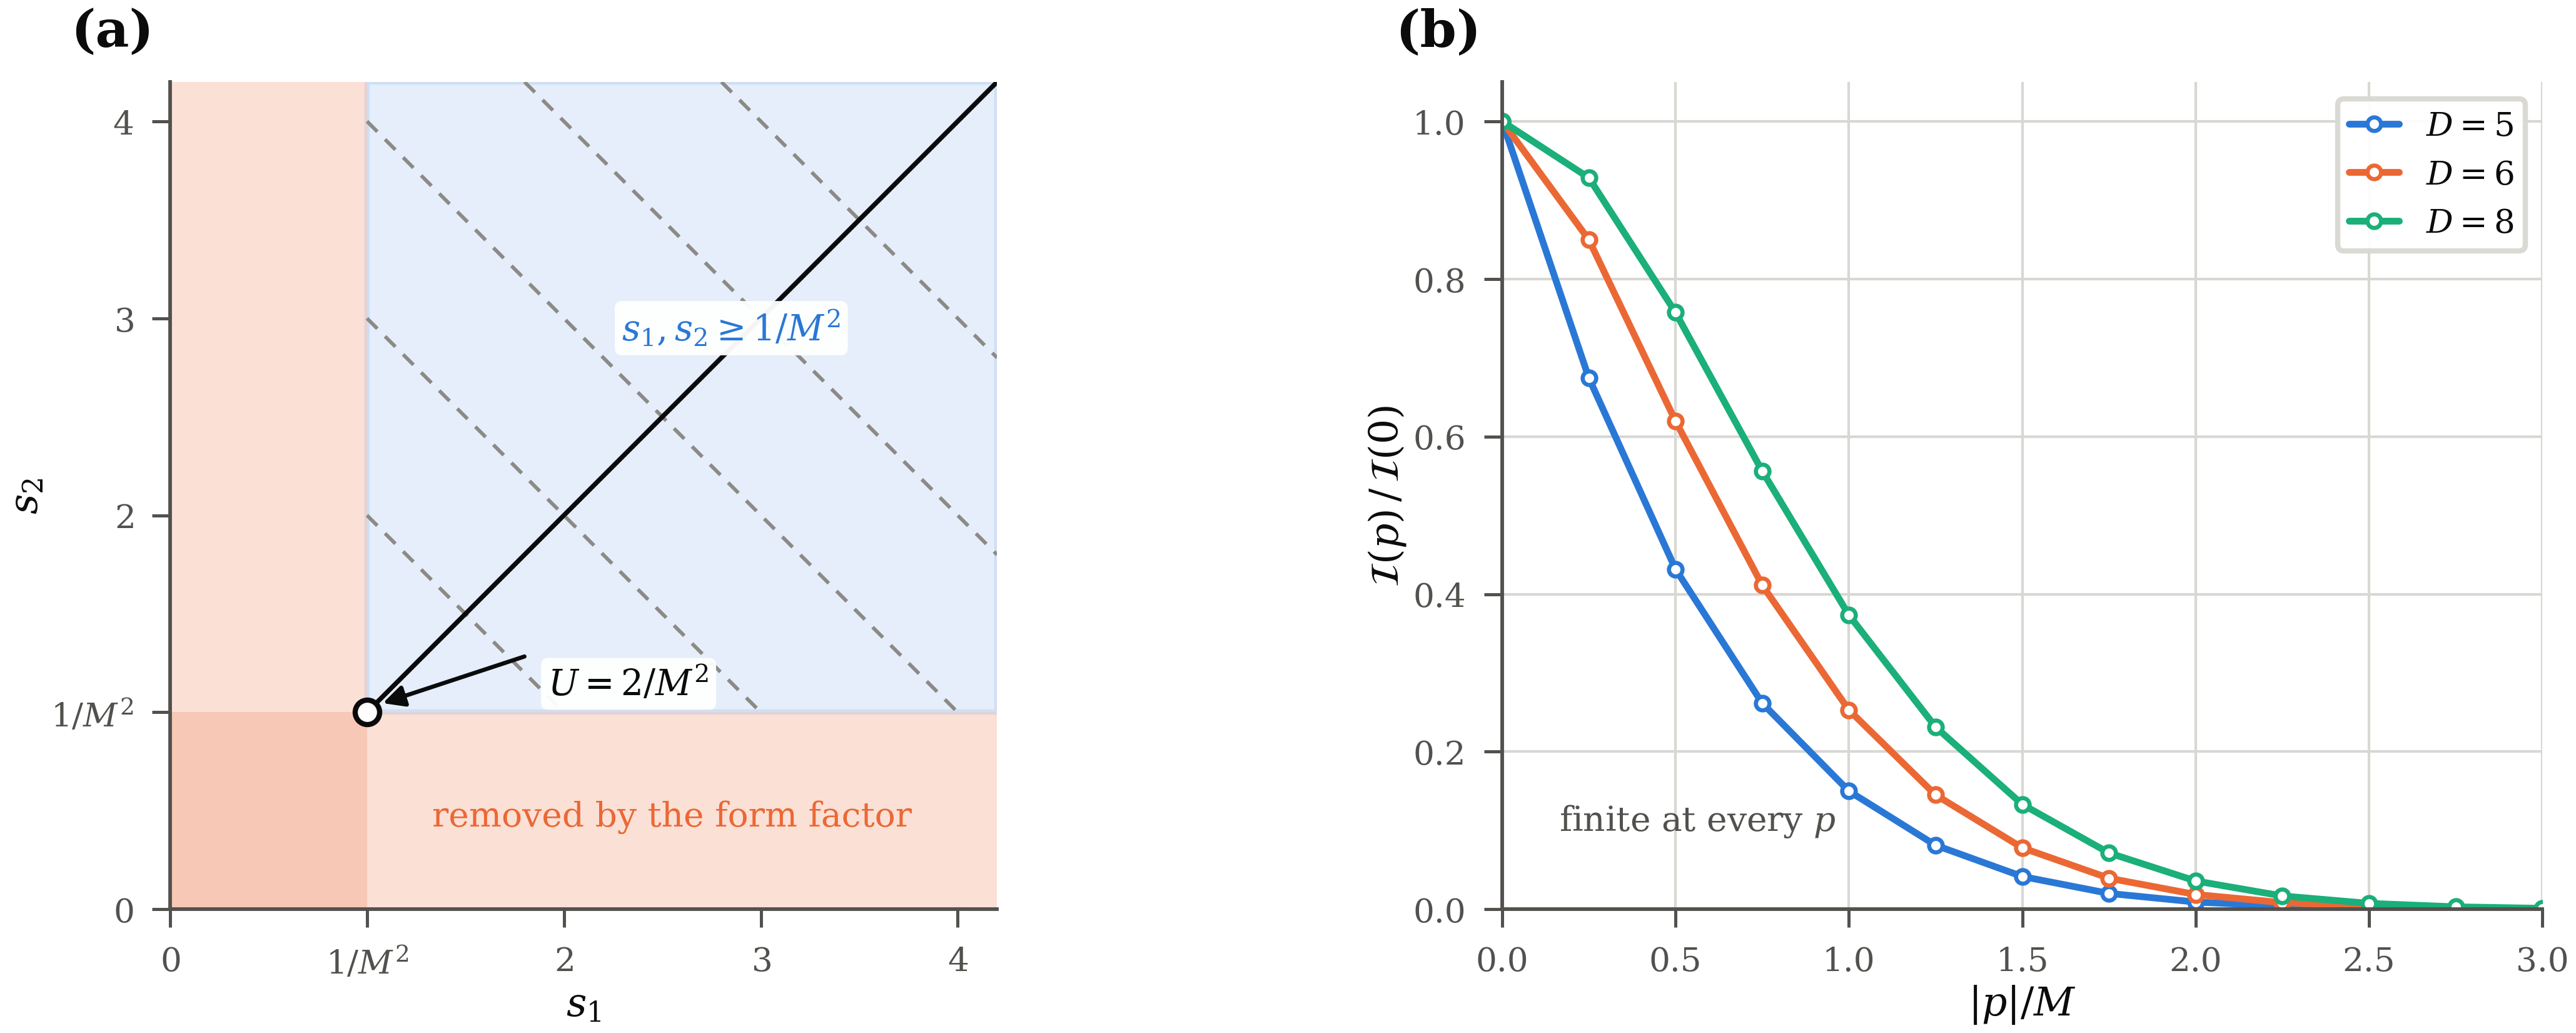
\includegraphics[width=\textwidth]{figs/fig06_schwinger.png}
\caption{The parametric domain of the one-loop bubble, \eqref{eq:bubble}. Dressing the propagators with $e^{-k^2/M^2}$ removes the shaded corner near the origin, where the ultraviolet divergence of the undressed graph comes from, and leaves the quadrant $s_1,s_2\ge1/M^2$. Along the diagonal $U=s_1+s_2$ attains its minimum $2/M^2$ on the domain, which is \eqref{eq:Ubound} for this graph. (b) The integral \eqref{eq:bubble}, normalized to its value at $p=0$, against the external momentum in $D=5,6,8$; it is finite at every $p$.}
\label{fig:schwinger}
\end{figure*}

\subsection{Position space}

\begin{theorem}[the Euclidean propagator]
\label{thm:GD}
In $D\ge3$ Euclidean dimensions the position-space propagator of $p^2e^{p^2/M^2}$ is
\begin{equation}
\label{eq:GD}
G_D(r)=\int\frac{\dd^Dp}{(2\pi)^D}\,\frac{e^{ip\cdot x}e^{-p^2/M^2}}{p^2}
=\frac{\gamma\bigl(\tfrac D2-1,\tfrac{M^2r^2}{4}\bigr)}{4\pi^{D/2}\,r^{D-2}},
\end{equation}
with $\gamma(s,x)=\int_0^x t^{s-1}e^{-t}\dd t$ the lower incomplete gamma function. It is smooth, positive, decreasing, equal to the massless propagator $\Gamma(\tfrac D2-1)/(4\pi^{D/2}r^{D-2})$ up to a relative error $\Gamma(\tfrac D2-1,\tfrac{M^2r^2}4)/\Gamma(\tfrac D2-1)$, and bounded at the origin by
\begin{equation}
\label{eq:G0}
G_D(0)=\frac{M^{D-2}}{2^{D-1}\pi^{D/2}(D-2)} .
\end{equation}
In particular $G_3(r)=\erf(Mr/2)/(4\pi r)$ and $G_4(r)=(1-e^{-M^2r^2/4})/(4\pi^2r^2)$, with $G_4(0)=M^2/(16\pi^2)$.
\end{theorem}

\begin{proof}
Write $e^{-p^2/M^2}/p^2=\int_0^\infty e^{-p^2(s+1/M^2)}\dd s$ and perform the Gaussian momentum integral,
\[
G_D(r)=\int_{1/M^2}^{\infty}(4\pi t)^{-D/2}e^{-r^2/4t}\,\dd t .
\]
The substitution $v=r^2/4t$ turns this into
\[
\frac{r^2}{4}(\pi r^2)^{-D/2}\int_0^{M^2r^2/4}v^{D/2-2}e^{-v}\,\dd v,
\]
which is \eqref{eq:GD}. Positivity, monotonicity and smoothness are read off the integral representation. As $r\to\infty$, $\gamma(s,x)\to\Gamma(s)$ and the difference is the upper incomplete gamma function. As $r\to0$, $\gamma(s,x)=x^s/s+O(x^{s+1})$, so $G_D(r)\to(M^2/4)^{D/2-1}/\bigl((D/2-1)4\pi^{D/2}\bigr)$, which is \eqref{eq:G0}. For $D=3$, $\gamma(\tfrac12,x)=\sqrt\pi\,\erf\sqrt x$; for $D=4$, $\gamma(1,x)=1-e^{-x}$.
\end{proof}

\begin{theorem}[Newtonian potential and the weak-field threshold]
\label{thm:potential}
In the static weak-field limit of the theory with $a(\Box)=e^{-\Box/M^2}$, the potential of a point mass $m$ is
\begin{equation}
\label{eq:potential}
\Phi(r)=-\frac{Gm}{r}\,\erf\Bigl(\frac{Mr}{2}\Bigr),
\end{equation}
which solves $\nabla^2\Phi=4\pi G\rho_{\mathrm{eff}}$ for the Gaussian source $\rho_{\mathrm{eff}}(r)=m(M/2)^3\pi^{-3/2}e^{-M^2r^2/4}$ of total mass $m$. It satisfies:
\begin{enumerate}[label=\textup{(\alph*)},leftmargin=2.2em,itemsep=0.1em]
\item the relative deviation from Newton's potential is $\erfc(Mr/2)$, which is below $10^{-3}$ for $Mr>4.654$ and below $10^{-11}$ for $Mr>10$;
\item $\Phi(0)=-GmM/\sqrt\pi$, and $\Phi(r)=-\frac{GmM}{\sqrt\pi}\bigl(1-\tfrac1{12}M^2r^2+O(M^4r^4)\bigr)$;
\item the enclosed mass of the effective source is $m\bigl[\erf(u)-\tfrac{2u}{\sqrt\pi}e^{-u^2}\bigr]$, $u=Mr/2$;
\item $\sup_r2|\Phi(r)|=2GmM/\sqrt\pi$, so the linearized field is weak everywhere, $2|\Phi|<1$, exactly when
\begin{equation}
\label{eq:threshold}
m<m_*=\frac{\sqrt\pi}{2GM} .
\end{equation}
\end{enumerate}
\end{theorem}

\begin{proof}
The linearized field equation in the static limit is $e^{-\nabla^2/M^2}\nabla^2\Phi=4\pi Gm\,\delta^3$, so $\widetilde\Phi(k)=-4\pi Gm\,e^{-k^2/M^2}/k^2$ and $\Phi=-4\pi Gm\,G_3$, which is \eqref{eq:potential} by Theorem~\ref{thm:GD}. Equivalently, $e^{-k^2/M^2}$ is the Fourier transform of the normalized Gaussian of width $2/M$, so $\Phi$ is the Newtonian potential of the smeared source $\rho_{\mathrm{eff}}$. (a) is the definition of $\erfc$ together with $\erfc(2.327)=10^{-3}$ and $\erfc(5)=1.5\times10^{-12}$. (b) follows from $\erf(x)=\frac{2}{\sqrt\pi}(x-x^3/3+\dots)$. (c) is the radial integral of $\rho_{\mathrm{eff}}$. For (d), $|\Phi|=GmM\,\erf(u)/(2u)$ with $u=Mr/2$, and $\frac{\dd}{\dd u}\bigl[\erf(u)/u\bigr]=\bigl(\tfrac{2u}{\sqrt\pi}e^{-u^2}-\erf(u)\bigr)/u^2<0$ for $u>0$, because $\erf(u)>\tfrac{2u}{\sqrt\pi}e^{-u^2}$ (both vanish at $0$ and the derivative of the difference is $\tfrac{4u^2}{\sqrt\pi}e^{-u^2}>0$); so $|\Phi|$ is strictly decreasing in $r$ and its supremum is the limit at $r=0$, $GmM/\sqrt\pi$.
\end{proof}

\begin{remark}
The threshold \eqref{eq:threshold} is the linearized shadow of the mass gap for horizon formation in ghost-free gravity found by Frolov \cite{Frolov2015}: below $m_*$ the metric function $1+2\Phi$ stays positive for every $r$ and no trapped surface forms in the weak-field description, above it $1+2\Phi$ crosses zero at some $r$ of order $1/M$, where the linearization is no longer trustworthy and the full nonlinear solution is needed; regular black hole metrics with Gaussian-smeared sources have been constructed in \cite{NicoliniSmailagicSpallucci2006,ModestoMoffatNicolini2011}. Nothing in the present paper depends on the nonlinear regime.
\end{remark}

\begin{proposition}[laboratory scale]
\label{prop:lab}
A measured agreement with the inverse-square law at separation $r$ to relative precision $\epsilon$ implies $M>(2/r)\erfc^{-1}(\epsilon)$. For $\epsilon=10^{-2}$ at $r=52\,\mu\mathrm m$, the smallest separation probed by the torsion-balance experiment of \cite{Lee2020}, this gives $1/M<14.3\,\mu\mathrm m$; a test at the same separation with $\epsilon=10^{-3}$ would give $1/M<11.2\,\mu\mathrm m$.
\end{proposition}

\begin{proof}
By Theorem~\ref{thm:potential}(a) the relative deviation from Newton's potential at separation $r$ is $\erfc(Mr/2)$, and $\erfc$ is decreasing; $\erfc^{-1}(10^{-2})=1.821$ and $\erfc^{-1}(10^{-3})=2.327$.
\end{proof}

The bound is stated for the potential; the force deviates by a different factor of the same order, and a dedicated fit of the Gaussian profile to the data of \cite{Lee2020}, which is analyzed there in terms of Yukawa corrections, would sharpen the number. The point of Proposition~\ref{prop:lab} is that the scale $M$ is constrained by short-distance experiments and by nothing else in this paper: in the wave zone the theory is indistinguishable from general relativity, as the next statement makes exact.

\begin{proposition}[exact luminality]
\label{prop:luminal}
Let $a=e^{H}$ with $H$ entire and $H(0)=0$. The spin-two propagator has its only pole at $p^2=0$, so the on-shell dispersion relation of the graviton is $\omega^2=k^2$ exactly, for every $k$: phase and group velocity are $1$, there is no birefringence and no massive branch. In particular the multi-messenger bound $|c_{\mathrm{gw}}/c-1|\lesssim10^{-15}$ of \cite{GW170817} is satisfied identically. A form factor of type (a) in Theorem~\ref{thm:dichotomy} with a real zero at $z=-M_1^2$ has instead a massive branch $\omega^2=k^2+M_1^2$ of residue $r_1<0$.
\end{proposition}

\begin{proof}
On-shell propagation is governed by the poles. By Theorem~\ref{thm:dichotomy}(b) the function $e^{-H(p^2)}/p^2$ has a single simple pole at $p^2=0$, so the on-shell condition is $p^2=0$, that is $\omega^2=k^2$ in Lorentzian signature, whatever $H$; both velocities are $1$, and the two helicities cannot separate because the form factor multiplies $\Pt$ by a scalar. In case (a) the pole at $z=-M_1^2$ gives the massive branch with the residue of Theorem~\ref{thm:sumrule}.
\end{proof}

The position-space side of the same form factor is drawn in Fig.~\ref{fig:propagator}: the propagator of Theorem~\ref{thm:GD} in four dimensions and its neighbours, the potential \eqref{eq:potential} against the Newtonian one, and the threshold \eqref{eq:threshold}.

\begin{figure*}[t]
\centering
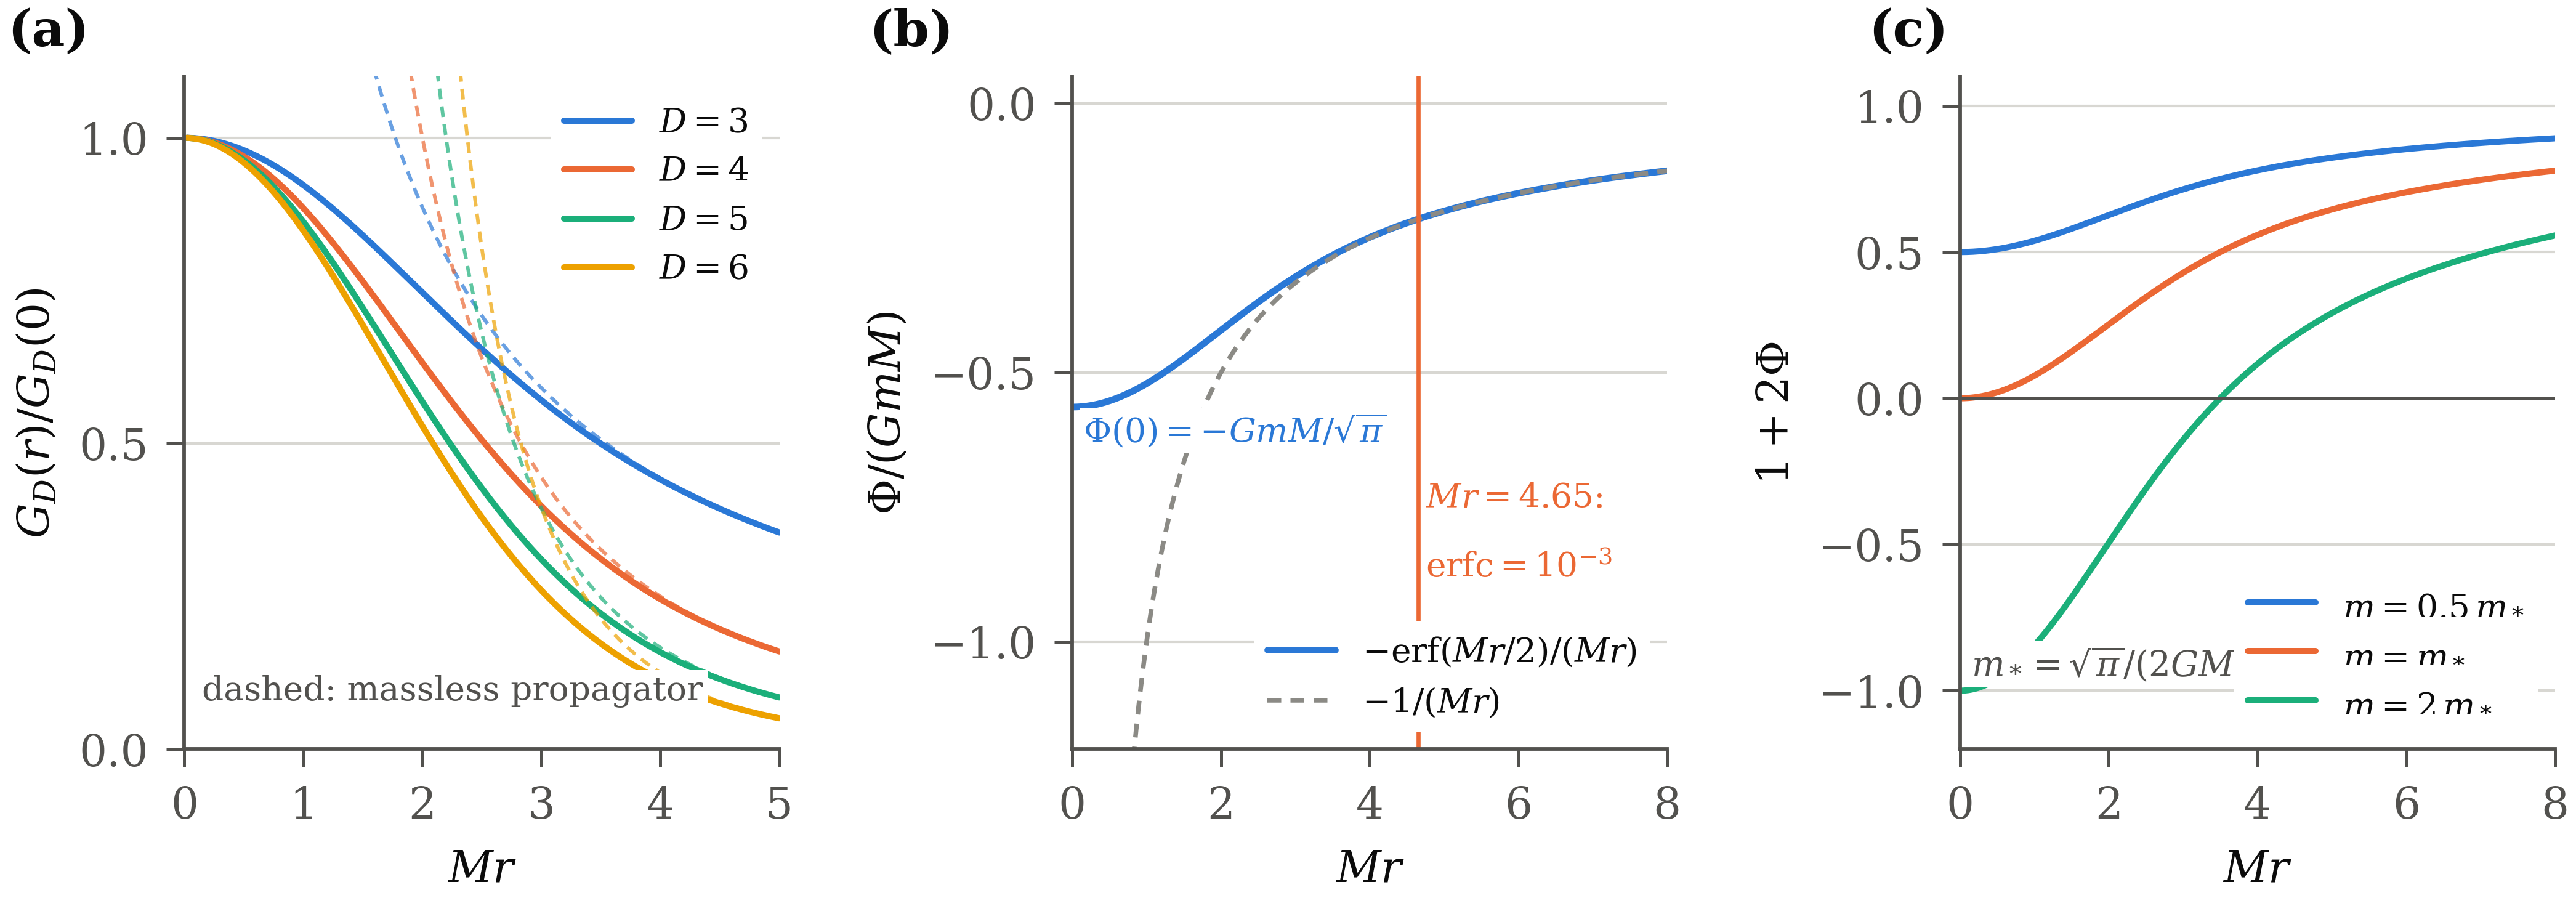
\includegraphics[width=\textwidth]{figs/fig05_propagator.png}
\caption{The Gaussian form factor in position space. (a) The Euclidean propagator $G_D$ of Theorem~\ref{thm:GD} in $D=3,4,5,6$, normalized by its value at the origin, against the massless propagator it approaches. (b) The Newtonian potential \eqref{eq:potential} against $-Gm/r$; the relative deviation $\erfc(Mr/2)$ drops below $10^{-3}$ at $Mr=4.65$. (c) The weak-field metric function $1+2\Phi$ for masses below, at and above the threshold $m_*=\sqrt\pi/(2GM)$ of Theorem~\ref{thm:potential}(d).}
\label{fig:propagator}
\end{figure*}

\section{One axis for the standard frameworks}
\label{sec:compare}

Whenever the graviton propagator has a definite large-momentum power, Theorem~\ref{thm:power} fixes the ultraviolet behavior and Theorem~\ref{thm:sumrule} fixes the pole content, so different frameworks can be set side by side. Table~\ref{tab:compare} does this; the propagator is $1/(p^2a(p^2))$ throughout, Einstein gravity diverges at every loop order, and the polynomial counting does not apply to the Gaussian form factor.

\begin{table}[htbp]
\caption{The ultraviolet behavior of each framework reduced to two columns: the degree of divergence $\omega(L)$ in $D=4$ and the pole content of the spin-two propagator. ``Truncated'' means a deterministic arrangement of $n$ weighted branes under Hypothesis~\ref{hyp:mult}, or any polynomial form factor of degree $n$.}
\label{tab:compare}
\begin{ruledtabular}
\begin{tabular}{lccl}
framework & $a(p^2)$ & $\omega(L)$ & poles \\
\colrule
Einstein & $1$ & $2+2L$ & none \\
Stelle $R^2$ & $1+p^2/M^2$ & $4$ & one, res.\ $-1$ \\
trunc., $n=2$ & degree $2$ & $6-2L$ & two, sum $-1$ \\
trunc., $n=3$ & degree $3$ & $8-4L$ & three, sum $-1$ \\
gas, growth $n$ & $e^{H}$ & $2{+}2n{+}(2{-}2n)L$ & none \\
gas, Gaussian & $e^{p^2/M^2}$ & none & none \\
\end{tabular}
\end{ruledtabular}
\end{table}

The last two rows are the only ones with no massive pole, and the fifth is the only one in which $\omega$ decreases with $L$ while the propagator keeps a single pole. Einstein gravity as an effective field theory \cite{Donoghue1994} occupies the first row with the understanding that the counterterms are organized by dimension rather than removed.

\section{Verification}
\label{sec:verification}

A program supplied with the manuscript recomputes every number quoted above from its definition, and a second one tests every figure for label collisions. The numerical suite runs $171$ checks in eleven groups. None of them takes a formula proved in the paper as an input.
\begin{enumerate}[label=\textup{(\arabic*)},leftmargin=2.4em,itemsep=0.1em]
\item The nerve complex: $\partial^2=0$ on the nerves of arrangements of up to eight hyperplanes in up to four dimensions and on random simplicial complexes; the two Euler sums of \eqref{eq:euler}; the census of Proposition~\ref{prop:census} for $D\in\{2,3,4,6,10,11,26\}$.
\item Intersection numbers: $[\bZ^D:M\bZ^D]=|\det M|$ on random integer matrices by enumeration of $M^{-1}\bZ^D/\bZ^D$; the two-torus law on all $960$ primitive pairs with entries in $[-3,3]$.
\item Generating functions: the subset sum \eqref{eq:cluster-sum} against the product for $N\in\{3,5,8\}$ and the location of the zeros; the Poisson identity \eqref{eq:pgfl} and the factorial moments by Monte Carlo over $4\times10^5$ realizations; the finiteness of $\log|e^{H}|$ on a grid for four entire $H$.
\item The projector algebra of Lemma~\ref{lem:projectors} on random momenta.
\item Residues: the sum rule \eqref{eq:sumrule} for $n\in\{1,2,3,5\}$ real masses and for complex conjugate pairs, the closed form \eqref{eq:residues}, the alternation, Stelle's partial fractions at three masses, and the residues $+1$ and $-1$ by contour integration.
\item Power counting: \eqref{eq:omega} against the direct count on $3000$ random $(V,L,n,D)$; the frontier for $2\le n\le39$; the census; $\omega(1)=4$; the threshold $n\ge D$ for $D\le11$; the rows of Table~\ref{tab:compare}.
\item The propagator: \eqref{eq:GD} against the radial Fourier integral in $D=3,4,5,6$ to $10^{-15}$; \eqref{eq:G0}; the closed forms in $D=3,4$; the Newtonian tail.
\item The potential: $\Phi(0)$, the Poisson equation with the Gaussian source to $10^{-7}$, the enclosed mass, the crossover values of $\erfc$, the monotonicity of $\erf(u)/u$, the threshold, and the laboratory number $14.3\,\mu$m.
\item Dispersion: $\omega=k$ on shell for three entire $H$, both velocities, and the subluminal group velocity of the massive branch of case (a).
\item The parametric representation: the Schwinger form \eqref{eq:schwinger} at nine values of $(M,k^2)$; the bound \eqref{eq:Ubound} for the bubble, the triangle, the sunset and the box, with the spanning-tree count taken from Kirchhoff's matrix-tree theorem and the corner verified to be the minimum over random interior points; the slice of the integrand at fixed $u=s_1+s_2$, evaluated as a Dawson function, against direct quadrature at nine values of $(u,p^2)$; the closed form \eqref{eq:bubble0} against the numerical integral in $D=5,6,8,10$ to a relative $10^{-9}$; and the finiteness of the $D=4$ bubble at $p^2>0$ together with its logarithmic growth as $p\to0$.
\item Composition of amplitudes: the single-brane case; the formula \eqref{eq:fabry} against the exact transfer matrix of two branes at four values of $(|r|,\delta)$, to a relative $10^{-12}$; the $|r|^2$ scaling of the error in \eqref{eq:product} for $N=3,5,8$, measured as a factor of $100$ per decade; its growth with the number of branes; and unitarity of the single brane.
\end{enumerate}
All $171$ checks pass.

The figure test renders each figure twice, with and without its text, intersects the bounding boxes of all pairs of labels inset by $1.5$ pixels, and measures the density of image edges under each label in the text-free rendering; labels with an opaque background are exempt. Every figure passes with zero flags.

\section{Discussion}
\label{sec:discussion}

Two statements do most of the work here, and they point in opposite directions. The first is the sum rule. A form factor with finitely many zeros produces massive poles whose residues add to $-1$, so a truncated cluster expansion, a finite arrangement of branes, or any polynomial improvement of the propagator pays for its power counting with a ghost, a tachyon or a complex pair. Reorganizing the perturbation series does not help, since the residues are read off the analytic function itself. The second is the exponential. A Poisson gas of branes with multiplicative couplings has, on average, the form factor $e^{H}$ with $H$ entire; an exponential has no zeros, the averaged propagator keeps its single pole, the graviton is massless and luminal at every wavenumber, and the classical potential is regular at the origin.

Three things are left unsettled. The first is unitarity beyond the tree-level residue. The factor $e^{-H}$ grows in some directions of the complex $p^2$ plane, so the usual Wick rotation and the usual Cutkosky rules need a prescription. Prescriptions that work have been given \cite{PiusSen2016,BrisceseModesto2019}, but we have not shown that any of them survives to all orders for an $H$ of the form a gas produces. Until that is done, the phrase ghost free should be read as it was defined in Sec.~\ref{sec:intro}, as a statement about the poles of the tree-level propagator.

The status of the average is the second. Since $e^{H}$ is the mean of the kinetic operator, it describes a gas whose fluctuations are fast compared with the graviton. A frozen gas gives instead an average of propagators, each with the poles of Proposition~\ref{prop:poly}, and averaging propagators does not remove the negative residues that Theorem~\ref{thm:sumrule} assigns to every realization. A derivation of the annealed effective action from a microscopic brane theory, with string theory the obvious candidate \cite{Polchinski1995,Johnson2003}, would decide this and also whether the fast-fluctuation regime is the physically relevant one. That derivation is the step the model most needs.

The scale is the third. In the wave zone the theory cannot be told apart from general relativity, so what constrains it is short-distance tests of the inverse-square law, through Proposition~\ref{prop:lab}. The value of $M$ is the integral $\int w\,\dd\Lambda$ over the gas, and the model does not fix it. Computing it for a particular gas, with a given intensity measure and coupling profile, is the most concrete task this paper leaves undone.

\section*{Data availability}

The data that support the findings of this study are contained in the manuscript. The source code that reproduces every numerical value quoted here and regenerates every figure is supplied with the article\ifzenodo{} and is archived at \href{https://doi.org/\zenododoi}{\nolinkurl{doi:\zenododoi}}\fi. It consists of \texttt{checks\_clusters.py}, which performs the $171$ checks itemized in Sec.~\ref{sec:verification}, together with \texttt{fig01\_arrangement.py} through \texttt{fig08\_annealed.py} and the shared module \texttt{figstyle.py}, which redraw Figs.~\ref{fig:arrangement} to \ref{fig:annealed} and rerun the label collision test. The scripts require \textsc{numpy}, \textsc{scipy} and \textsc{matplotlib}, and take no other input.

\section*{Funding}

This research received no specific grant from any funding agency in the public, commercial or not-for-profit sectors.

\section*{Conflict of interest}

The authors declare no conflict of interest.

\begin{acknowledgments}
Every digital object identifier in the bibliography was resolved against the registration record of the item before inclusion.
\end{acknowledgments}

\appendix

\section{Conventions}
\label{app:conventions}

Spacetime is $D$-dimensional. The momentum-space computations are done in Euclidean signature, where $p^2\ge0$ and the poles of the propagator lie on the negative real axis of the complex $p^2$ plane; the Lorentzian statements follow by the usual rotation and none of the counting changes, because the number and residues of the poles are properties of the entire function $a$ and not of the contour. The curvature conventions are $R^\rho{}_{\sigma\mu\nu}=\partial_\mu\Gamma^\rho_{\nu\sigma}-\partial_\nu\Gamma^\rho_{\mu\sigma}+\cdots$, $R_{\mu\nu}=R^\rho{}_{\mu\rho\nu}$, so that spheres have positive scalar curvature; $\Box=g^{\mu\nu}\nabla_\mu\nabla_\nu$ and $\kappa^2=32\pi G$. A brane is oriented and a transverse intersection carries the orientation for which the orientation of $B_S$ followed by the normals of the branes in $S$, in order, agrees with the orientation of $X$; this fixes the sign of \eqref{eq:detM} up to the absolute value.

\section{Variation of the form-factor term}
\label{app:stress}

For a scalar field $\phi$ with the nonlocal term $S_a=-\tfrac12\int\sqrt g\,\phi\,a(\Box)\phi$, $a(\Box)=\sum_{j\ge0}c_j\Box^j$, the variation with respect to $g^{\mu\nu}$ produces, from the $j$-th term and the Leibniz rule applied $j$ times,
\begin{multline}
\label{eq:Theta}
\Theta_{\mu\nu}=-\tfrac12\sum_{j\ge1}c_j\sum_{l=0}^{j-1}\Bigl[\nabla_\mu(\Box^l\phi)\nabla_\nu(\Box^{j-l-1}\phi)\\
-\tfrac12g_{\mu\nu}\nabla^\alpha(\Box^l\phi)\nabla_\alpha(\Box^{j-l-1}\phi)\Bigr]
-\tfrac12g_{\mu\nu}\sum_{j\ge0}c_j\,\phi\Box^j\phi ,
\end{multline}
up to total derivatives. The series converges wherever the series of $a$ does, hence everywhere for an entire $a$, and the divergence of \eqref{eq:Theta} telescopes: the $l$-th term of the inner sum cancels the $(l+1)$-st after one integration by parts, leaving the equation-of-motion term $-\nabla_\nu\phi\,\delta S_a/\delta\phi$, which is the Noether identity that makes the total stress tensor conserved on shell. The graviton case is the same computation with $h_{\mu\nu}$ in place of $\phi$ and the projectors of Lemma~\ref{lem:projectors} carried along; it fixes the vertex form factors in terms of the propagator form factor assumed in Hypothesis~\ref{hyp:growth}.

\section{Poisson identities}
\label{app:poisson}

For a Poisson process $\Pi$ with finite intensity measure $\Lambda$ on $\mathcal S$ and a bounded measurable $f:\mathcal S\to\bC$, the probability generating functional is $\bE\prod_{x\in\Pi}(1+f(x))=\exp\int f\,\dd\Lambda$, and the $K$-th factorial moment measure, defined by $\bE\sum_{(x_1,\dots,x_K)}g(x_1,\dots,x_K)$ over $K$-tuples of distinct points, is $\Lambda^{\otimes K}$ \cite[Chapters 3 and 4]{LastPenrose2017}, \cite{Kingman1993}. Both identities were used in Theorem~\ref{thm:poisson}, and both follow from the representation of the process by a Poisson number of independent points. For a stationary Poisson process of hyperplanes in $\bR^D$ the intersection strata form the Poisson flat processes of stochastic geometry, whose intensities are given by the same factorial moments with geometric weights \cite[Chapter~4]{SchneiderWeil2008}; the intensity of the $K$-fold intersection process of a process of hyperplanes with intensity $\gamma$ is $\gamma^K/K!$ times the expected volume of the parallelepiped spanned by $K$ independent unit normals drawn from the direction distribution. Figure~\ref{fig:arrangement}(b) is a sample of such a process, and the expected numbers of its lines and of its points in a fixed box are, up to these geometric factors, $\Lambda^2/2$ and $\Lambda^3/6$ with $\Lambda$ the expected number of planes.

\makeatletter
\renewcommand\bibcite[2]{\global\@namedef{b@#1\@extra@binfo}{#2}}
\makeatother
\begin{thebibliography}{99}

\bibitem{tHooftVeltman1974}
G.~'t~Hooft and M.~Veltman, One-loop divergencies in the theory of gravitation, Ann. Inst. H. Poincar\'e Sect. A \textbf{20}, 69 (1974), \url{http://www.numdam.org/item/AIHPA_1974__20_1_69_0/}.

\bibitem{GoroffSagnotti1986}
M.~H. Goroff and A.~Sagnotti, The ultraviolet behavior of Einstein gravity, Nucl. Phys. B \textbf{266}, 709 (1986), \href{https://doi.org/10.1016/0550-3213(86)90193-8}{\nolinkurl{doi:10.1016/0550-3213(86)90193-8}}.

\bibitem{Stelle1977}
K.~S. Stelle, Renormalization of higher-derivative quantum gravity, Phys. Rev. D \textbf{16}, 953 (1977), \href{https://doi.org/10.1103/PhysRevD.16.953}{\nolinkurl{doi:10.1103/PhysRevD.16.953}}.

\bibitem{Weinberg1979}
S.~Weinberg, Ultraviolet divergences in quantum theories of gravitation, in \emph{General Relativity: An Einstein Centenary Survey}, edited by S.~W. Hawking and W.~Israel (Cambridge University Press, Cambridge, 1979), pp.~790--831.

\bibitem{Reuter1998}
M.~Reuter, Nonperturbative evolution equation for quantum gravity, Phys. Rev. D \textbf{57}, 971 (1998), \href{https://doi.org/10.1103/PhysRevD.57.971}{\nolinkurl{doi:10.1103/PhysRevD.57.971}}.

\bibitem{Efimov1967}
G.~V. Efimov, Non-local quantum theory of the scalar field, Commun. Math. Phys. \textbf{5}, 42 (1967), \href{https://doi.org/10.1007/BF01646357}{\nolinkurl{doi:10.1007/BF01646357}}.

\bibitem{Krasnikov1987}
N.~V. Krasnikov, Nonlocal gauge theories, Theor. Math. Phys. \textbf{73}, 1184 (1987), \href{https://doi.org/10.1007/BF01017588}{\nolinkurl{doi:10.1007/BF01017588}}.

\bibitem{Kuzmin1989}
Yu.~V. Kuzmin, Finite nonlocal gravity, Sov. J. Nucl. Phys. \textbf{50}, 1011 (1989).

\bibitem{Tomboulis1997}
E.~T. Tomboulis, Superrenormalizable gauge and gravitational theories, arXiv:hep-th/9702146 (1997), \href{https://doi.org/10.48550/arXiv.hep-th/9702146}{\nolinkurl{doi:10.48550/arXiv.hep-th/9702146}}.

\bibitem{BiswasMazumdarSiegel2006}
T.~Biswas, A.~Mazumdar, and W.~Siegel, Bouncing universes in string-inspired gravity, J. Cosmol. Astropart. Phys. \textbf{03} (2006) 009, \href{https://doi.org/10.1088/1475-7516/2006/03/009}{\nolinkurl{doi:10.1088/1475-7516/2006/03/009}}.

\bibitem{BGKM2012}
T.~Biswas, E.~Gerwick, T.~Koivisto, and A.~Mazumdar, Towards singularity- and ghost-free theories of gravity, Phys. Rev. Lett. \textbf{108}, 031101 (2012), \href{https://doi.org/10.1103/PhysRevLett.108.031101}{\nolinkurl{doi:10.1103/PhysRevLett.108.031101}}.

\bibitem{Modesto2012}
L.~Modesto, Super-renormalizable quantum gravity, Phys. Rev. D \textbf{86}, 044005 (2012), \href{https://doi.org/10.1103/PhysRevD.86.044005}{\nolinkurl{doi:10.1103/PhysRevD.86.044005}}.

\bibitem{Foldy1945}
L.~L. Foldy, The multiple scattering of waves. I. General theory of isotropic scattering by randomly distributed scatterers, Phys. Rev. \textbf{67}, 107 (1945), \href{https://doi.org/10.1103/PhysRev.67.107}{\nolinkurl{doi:10.1103/PhysRev.67.107}}.

\bibitem{Lax1951}
M.~Lax, Multiple scattering of waves, Rev. Mod. Phys. \textbf{23}, 287 (1951), \href{https://doi.org/10.1103/RevModPhys.23.287}{\nolinkurl{doi:10.1103/RevModPhys.23.287}}.

\bibitem{Frolov2015}
V.~P. Frolov, Mass-gap for black hole formation in higher-derivative and ghost-free gravity, Phys. Rev. Lett. \textbf{115}, 051102 (2015), \href{https://doi.org/10.1103/PhysRevLett.115.051102}{\nolinkurl{doi:10.1103/PhysRevLett.115.051102}}.

\bibitem{Bhattacharjee2025brane}
S.~Singha Roy, R.~Sadhu, D.~Bhattacharjee, P.~Samal, P.~Nandi, and S.~N. Thakur, Brane clustering as a UV completion to quantum gravity, Preprints.org (2025), preprints202508.0407, version 2, \href{https://doi.org/10.20944/preprints202508.0407.v2}{\nolinkurl{doi:10.20944/preprints202508.0407.v2}}.

\bibitem{Bauer2023}
U.~Bauer, M.~Kerber, F.~Roll, and A.~Rolle, A unified view on the functorial nerve theorem and its variations, Expo. Math. \textbf{41}, 125503 (2023), \href{https://doi.org/10.1016/j.exmath.2023.04.005}{\nolinkurl{doi:10.1016/j.exmath.2023.04.005}}.

\bibitem{Cohen1993}
H.~Cohen, \emph{A Course in Computational Algebraic Number Theory}, Graduate Texts in Mathematics Vol.~138 (Springer, Berlin, 1993), \href{https://doi.org/10.1007/978-3-662-02945-9}{\nolinkurl{doi:10.1007/978-3-662-02945-9}}.

\bibitem{BottTu1982}
R.~Bott and L.~W. Tu, \emph{Differential Forms in Algebraic Topology}, Graduate Texts in Mathematics Vol.~82 (Springer, New York, 1982), \href{https://doi.org/10.1007/978-1-4757-3951-0}{\nolinkurl{doi:10.1007/978-1-4757-3951-0}}.

\bibitem{Kingman1993}
J.~F.~C. Kingman, \emph{Poisson Processes}, Oxford Studies in Probability Vol.~3 (Oxford University Press, Oxford, 1993).

\bibitem{LastPenrose2017}
G.~Last and M.~Penrose, \emph{Lectures on the Poisson Process}, Institute of Mathematical Statistics Textbooks Vol.~7 (Cambridge University Press, Cambridge, 2017), \href{https://doi.org/10.1017/9781316104477}{\nolinkurl{doi:10.1017/9781316104477}}.

\bibitem{Rivers1964}
R.~J. Rivers, Lagrangian theory for neutral massive spin-2 fields, Nuovo Cimento \textbf{34}, 386 (1964), \href{https://doi.org/10.1007/BF02734585}{\nolinkurl{doi:10.1007/BF02734585}}.

\bibitem{VanNieuwenhuizen1973}
P.~van Nieuwenhuizen, On ghost-free tensor Lagrangians and linearized gravitation, Nucl. Phys. B \textbf{60}, 478 (1973), \href{https://doi.org/10.1016/0550-3213(73)90194-6}{\nolinkurl{doi:10.1016/0550-3213(73)90194-6}}.

\bibitem{BarnichBrandtHenneaux2000}
G.~Barnich, F.~Brandt, and M.~Henneaux, Local BRST cohomology in gauge theories, Phys. Rep. \textbf{338}, 439 (2000), \href{https://doi.org/10.1016/S0370-1573(00)00049-1}{\nolinkurl{doi:10.1016/S0370-1573(00)00049-1}}.

\bibitem{Hadamard1893}
J.~Hadamard, \'Etude sur les propri\'et\'es des fonctions enti\`eres et en particulier d'une fonction consid\'er\'ee par Riemann, J. Math. Pures Appl. (4) \textbf{9}, 171 (1893).

\bibitem{Conway1978}
J.~B. Conway, \emph{Functions of One Complex Variable I}, 2nd ed., Graduate Texts in Mathematics Vol.~11 (Springer, New York, 1978), \href{https://doi.org/10.1007/978-1-4612-6313-5}{\nolinkurl{doi:10.1007/978-1-4612-6313-5}}.

\bibitem{Shapiro2015}
I.~L. Shapiro, Counting ghosts in the ``ghost-free'' non-local gravity, Phys. Lett. B \textbf{744}, 67 (2015), \href{https://doi.org/10.1016/j.physletb.2015.03.037}{\nolinkurl{doi:10.1016/j.physletb.2015.03.037}}.

\bibitem{Anselmi2017}
D.~Anselmi, On the quantum field theory of the gravitational interactions, J. High Energy Phys. \textbf{06} (2017) 086, \href{https://doi.org/10.1007/JHEP06(2017)086}{\nolinkurl{doi:10.1007/JHEP06(2017)086}}.

\bibitem{AnselmiPiva2017}
D.~Anselmi and M.~Piva, Perturbative unitarity of Lee--Wick quantum field theory, Phys. Rev. D \textbf{96}, 045009 (2017), \href{https://doi.org/10.1103/PhysRevD.96.045009}{\nolinkurl{doi:10.1103/PhysRevD.96.045009}}.

\bibitem{AsoreyLopezShapiro1997}
M.~Asorey, J.~L. L\'opez, and I.~L. Shapiro, Some remarks on high derivative quantum gravity, Int. J. Mod. Phys. A \textbf{12}, 5711 (1997), \href{https://doi.org/10.1142/S0217751X97002991}{\nolinkurl{doi:10.1142/S0217751X97002991}}.

\bibitem{Ostrogradsky1850}
M.~Ostrogradsky, M\'emoires sur les \'equations diff\'erentielles relatives au probl\`eme des isop\'erim\`etres, Mem. Acad. St. P\'etersbourg \textbf{6}, 385 (1850).

\bibitem{Woodard2015}
R.~P. Woodard, Ostrogradsky's theorem on Hamiltonian instability, Scholarpedia \textbf{10}, 32243 (2015), \href{https://doi.org/10.4249/scholarpedia.32243}{\nolinkurl{doi:10.4249/scholarpedia.32243}}.

\bibitem{ModestoRachwal2014}
L.~Modesto and L.~Rachwa{\l}, Super-renormalizable and finite gravitational theories, Nucl. Phys. B \textbf{889}, 228 (2014), \href{https://doi.org/10.1016/j.nuclphysb.2014.10.015}{\nolinkurl{doi:10.1016/j.nuclphysb.2014.10.015}}.

\bibitem{Talaganis2015}
S.~Talaganis, T.~Biswas, and A.~Mazumdar, Towards understanding the ultraviolet behavior of quantum loops in infinite-derivative theories of gravity, Classical Quantum Gravity \textbf{32}, 215017 (2015), \href{https://doi.org/10.1088/0264-9381/32/21/215017}{\nolinkurl{doi:10.1088/0264-9381/32/21/215017}}.

\bibitem{Smirnov2006}
V.~A. Smirnov, \emph{Feynman Integral Calculus} (Springer, Berlin, 2006), \href{https://doi.org/10.1007/3-540-30611-0}{\nolinkurl{doi:10.1007/3-540-30611-0}}.

\bibitem{Vassilevich2003}
D.~V. Vassilevich, Heat kernel expansion: user's manual, Phys. Rep. \textbf{388}, 279 (2003), \href{https://doi.org/10.1016/j.physrep.2003.09.002}{\nolinkurl{doi:10.1016/j.physrep.2003.09.002}}.

\bibitem{EdholmKoshelevMazumdar2016}
J.~Edholm, A.~S. Koshelev, and A.~Mazumdar, Behavior of the Newtonian potential for ghost-free gravity and singularity free gravity, Phys. Rev. D \textbf{94}, 104033 (2016), \href{https://doi.org/10.1103/PhysRevD.94.104033}{\nolinkurl{doi:10.1103/PhysRevD.94.104033}}.

\bibitem{Buoninfante2018}
L.~Buoninfante, A.~S. Koshelev, G.~Lambiase, and A.~Mazumdar, Classical properties of non-local, ghost- and singularity-free gravity, J. Cosmol. Astropart. Phys. \textbf{09} (2018) 034, \href{https://doi.org/10.1088/1475-7516/2018/09/034}{\nolinkurl{doi:10.1088/1475-7516/2018/09/034}}.

\bibitem{NicoliniSmailagicSpallucci2006}
P.~Nicolini, A.~Smailagic, and E.~Spallucci, Noncommutative geometry inspired Schwarzschild black hole, Phys. Lett. B \textbf{632}, 547 (2006), \href{https://doi.org/10.1016/j.physletb.2005.11.004}{\nolinkurl{doi:10.1016/j.physletb.2005.11.004}}.

\bibitem{ModestoMoffatNicolini2011}
L.~Modesto, J.~W. Moffat, and P.~Nicolini, Black holes in an ultraviolet complete quantum gravity, Phys. Lett. B \textbf{695}, 397 (2011), \href{https://doi.org/10.1016/j.physletb.2010.11.046}{\nolinkurl{doi:10.1016/j.physletb.2010.11.046}}.

\bibitem{Lee2020}
J.~G. Lee, E.~G. Adelberger, T.~S. Cook, S.~M. Fleischer, and B.~R. Heckel, New test of the gravitational $1/r^2$ law at separations down to 52 $\mu$m, Phys. Rev. Lett. \textbf{124}, 101101 (2020), \href{https://doi.org/10.1103/PhysRevLett.124.101101}{\nolinkurl{doi:10.1103/PhysRevLett.124.101101}}.

\bibitem{GW170817}
B.~P. Abbott \emph{et al.} (LIGO Scientific Collaboration, Virgo Collaboration, Fermi GBM, and INTEGRAL), Gravitational waves and gamma-rays from a binary neutron star merger: GW170817 and GRB 170817A, Astrophys. J. Lett. \textbf{848}, L13 (2017), \href{https://doi.org/10.3847/2041-8213/aa920c}{\nolinkurl{doi:10.3847/2041-8213/aa920c}}.

\bibitem{Donoghue1994}
J.~F. Donoghue, General relativity as an effective field theory: the leading quantum corrections, Phys. Rev. D \textbf{50}, 3874 (1994), \href{https://doi.org/10.1103/PhysRevD.50.3874}{\nolinkurl{doi:10.1103/PhysRevD.50.3874}}.

\bibitem{PiusSen2016}
R.~Pius and A.~Sen, Cutkosky rules for superstring field theory, J. High Energy Phys. \textbf{10} (2016) 024, \href{https://doi.org/10.1007/JHEP10(2016)024}{\nolinkurl{doi:10.1007/JHEP10(2016)024}}.

\bibitem{BrisceseModesto2019}
F.~Briscese and L.~Modesto, Cutkosky rules and perturbative unitarity in Euclidean nonlocal quantum field theories, Phys. Rev. D \textbf{99}, 104043 (2019), \href{https://doi.org/10.1103/PhysRevD.99.104043}{\nolinkurl{doi:10.1103/PhysRevD.99.104043}}.

\bibitem{Polchinski1995}
J.~Polchinski, Dirichlet branes and Ramond--Ramond charges, Phys. Rev. Lett. \textbf{75}, 4724 (1995), \href{https://doi.org/10.1103/PhysRevLett.75.4724}{\nolinkurl{doi:10.1103/PhysRevLett.75.4724}}.

\bibitem{Johnson2003}
C.~V. Johnson, \emph{D-Branes}, Cambridge Monographs on Mathematical Physics (Cambridge University Press, Cambridge, 2002), \href{https://doi.org/10.1017/CBO9780511606540}{\nolinkurl{doi:10.1017/CBO9780511606540}}.

\bibitem{SchneiderWeil2008}
R.~Schneider and W.~Weil, \emph{Stochastic and Integral Geometry}, Probability and Its Applications (Springer, Berlin, 2008), \href{https://doi.org/10.1007/978-3-540-78859-1}{\nolinkurl{doi:10.1007/978-3-540-78859-1}}.

\end{thebibliography}

\end{document}
